% !TeX spellcheck = fr_FR
\begin{resume}
Dans l'ensemble des éléments qui composent les systèmes informatiques, les réseaux d'interconnexion sont parmi les éléments qui sont les plus exposés et les plus impactés par l'hétérogénéité. Cette hétérogénéité peut se présenter sous différentes formes : diversité d'équipements et de technologies, variations de performance et de disponibilité (volatilité), limitations liées aux caractéristiques physiques ou à la capacité des ressources, etc. 

Si cette hétérogénéité doit être prise en compte lors du développement de systèmes et d'applications, il s'avère souvent que les solutions se limitent à pallier les éventuels problèmes. Parmi les travaux que j'ai mené dans le domaine de l'hétérogénéité des réseaux, on trouve souvent l'association entre l'observation (mesure des performances) et la modélisation (prédiction des performances). Ces deux facettes de la recherche visent la compréhension des facteurs liés à l'hétérogénéité, leur caractérisation et aussi l'optimisation des algorithmes de communication.

Dans ce sens, je me suis orienté vers l'étude et la modélisation des primitives de communication collective dans les réseaux hétérogènes de type \textit{grid}. Contrairement aux communications réseaux point à point (\textit{unicast}), les communications collectives visent la diffusion ou  la collecte de messages auprès un ensemble de n{\oe}uds. Parmi les patrons de communication collective nous trouvons celui dit \textit{one-to-many}, qui représente une diffusion (\textit{broadcast/multicast}), mais aussi des patrons plus élaborés tels que \textit{many-to-many} qui représente un échange total entre les n{\oe}uds : chaque n{\oe}ud a un message différent à envoyer à chacun des autres n{\oe}uds du réseau. 

Les travaux présentés ici concernent les développements effectués à la fin de mes travaux de thèse et poursuivis lors de mes activités en tant que ATER à Nancy, entre 2005 et 2007, période dans laquelle j'ai intégré l'Équipe ALGORILLE de l'INRIA Lorraine. Dans le même registre, il faut rajouter des collaborations autour de la modélisation des performances des algorithmes parallèles de multiplication matricielle avec le professeur Wahid Nasri de l'ESSTT (Tunisie) ou des développements sur le \textit{broadcast} pour les \textit{grids} dans le cadre de la thèse de doctorat de Hazem Fkaier (Université Paris 13).


%Cette première partie regroupe les travaux que j'ai menés sur la
%structuration des systèmes distribués à l'aide de marches
%aléatoires. Ils constituent la continuité de ceux menés durant ma
%thèse.
%
%J'exploite les marches aléatoires selon deux axes. Le premier consiste
%à n'utiliser que la circulation, sans collecte d'informations au cours
%du déplacement. Le second consiste à combiner les concepts de marche
%aléatoire et de mot circulant, afin d'exploiter l'historique des
%déplacements du jeton.
%
%La première approche m'a permis de définir un algorithme rapide de
%construction et de maintenance d'un arbre couvrant sur un système
%distribué. Cette construction est auto-stabili\-sante, et garantit
%donc la tolérance aux fautes transitoires qui peuvent affecter le
%système.
%
%Dans la seconde approche, l'historique des déplacements est conservé
%dans le jeton, mais n'a aucun impact sur la circulation qui reste
%aléatoire sans mémoire. Le contenu du jeton est analysé et exploité,
%afin de permettre la construction d'arbres couvrants sur chaque
%site. Je propose différents algorithmes auto-stabilisants de gestion
%et de correction du contenu du jeton et de sa circulation. Je dérive
%de cette circulation un algorithme auto-stabilisant garantissant la
%$k-$exclusion mutuelle.
%
%La majorité des travaux présentés dans cette partie, ont été réalisés
%en collaboration avec Alain Bui, professeur à l'université de Reims
%Champagne-Ardenne, et Thibault Bernard, dont je co-encadre une partie
%des travaux de thèse avec Alain Bui.

\end{resume}

\section{Modélisation des Performances d'un Réseau\label{sec:reseaux-model}}

%Dans le contexte de la modélisation de performance, nous appelons
%modèle la description formelle de l'exécution d'un programme sur une
%ou plusieurs machines, de manière à ce que cette description peut
%être utilisée pour comprendre, voire décrire, la performance de tel
%programme.

Une des meilleures manières de comprendre le fonctionnement des algorithmes
distribués et d'évaluer leur efficacité est de modéliser leur performance. Si d'un côté des facteurs non
déterministes influencent la performance des applications,
comme par exemple la congestion des ressources, pour la plupart du
temps leur impact sur le temps d'exécution est suffisamment
limité \cite{Grove03}. Ainsi, la plus grande difficulté pour la modélisation
des performances est la correcte représentation des facteurs liés
à la communication.  

Si les principes de la modélisation de performance peuvent être trouvés
dans des travaux pionniers des années 60 et 70 \cite{Peterson81},
la modélisation de performance a connu une importante attention à
partir des années 80, où des efforts importants ont été faits pour
identifier des modèles de performance adaptés aux technologies et aux
paradigmes qui ont surgi depuis la décennie précédente. Pour cette
raison, dans ce chapitre nous voulons identifier les modèles qui ont les caractéristiques
les plus adaptées à la modélisation réaliste des communications.


\subsection{Exécution dans les Systèmes Distribués : définitions}

Un système distribué peut être défini comme un ensemble
d'unités de traitement ou de calcul indépendantes, reliées entre elles
par des liens de communications. Ces unités de traitement contribuent
au calcul d'un résultat en effectuant leurs exécutions de façon
concurrente.

Un réseau d'interconnexion {\cal R}, aussi appelé système distribué,
est représenté par un graphe $G =(V,E)$, dans lequel $V$ est
l'ensemble des n{\oe}uds et $E$ l'ensemble des arêtes qui représente  les
liens ou les canaux de communication entre les n{\oe}uds.

%Par la suite, on parlera indifféremment de n{\oe}ud, de site, de
%processus ou de processeur pour définir un n{\oe}ud du réseau. De
%même, on parlera indifféremment de canaux ou de liens de communication
%pour définir les supports de la communication qu'utilise le réseau.

L'écriture d'un algorithme, ainsi que l'évaluation de ses
performances, ne peut se faire que si on a défini un
modèle d'exécution au préalable. Parmi les modèles existants dans la littérature,  celui que nous adoptons est modèle à passage de messages. Le modèle à passage de messages définit des canaux de communication
par lesquels transitent les messages. Il nécessite toutefois de poser des
hypothèses sur les propriétés des canaux de communication : capacité (débit),
délais de transmission (latence), caractéristiques des échanges...

Dans notre cas spécifique, nous voulons explorer le modèle à passage de messages afin d'apporter à la fois une
représentation fidèle du comportement des communications mais aussi une 
utilisation simple, capable d'être appliquée aux des environnements hétérogènes. Différents abstractions permettent la modélisation des communications avec plus ou moins de détails, ainsi la prochaine section passera en revue certaines modèles que nous avons étudié.


\subsection{Modélisation des Communications}

Le modèle de Hockney \cite{Hockney94} est un des plus utilisés pour
décrire la communication point-à-point dans les machines parallèles
à mémoire distribuée. Selon ce modèle, une communication entre deux
n{\oe}uds est décrite par : 

\[
t=t_{0}+\frac{m}{r_{\infty}}\]


où $t_{0}$ représente le temps nécessaire à l'envoi d'un message
de taille zéro, \emph{m} est la taille du message (en octets) et $r_{\infty}$
est le débit asymptotique en Moctets/s, i.e., le débit maximal obtenu
quand la taille du message s'approche de l'infini. Dans ce raisonnement,
$m/r_{\infty}$ représente le délai de transmission d'un message de
\emph{m} octets à travers un réseau avec un débit asymptotique de
$r_{\infty}$ Moctets/s.

Ce modèle est souvent transformé dans l'équation affine 

\[
t=\alpha+\beta m\]


où $\alpha$ correspond à la latence de transmission et $\beta$ est
le temps de transfert d'un octet sur ce réseau \cite{Pjesivac-Grbovic05}.
L'obtention des paramètres $\alpha$ et $\beta$ peut se faire à travers
l'utilisation de certains outils comme NWS \cite{Wolski97}. 

Toutefois, un inconvénient de ce modèle est qu'il assume que le temps
de transfert est proportionnel à la taille du message. Dans des situations
réelles, certains facteurs comme la taille de la mémoire tampon et
la segmentation des messages en paquets font varier le temps de transfert
$\beta$ selon la taille du message. 

À partir de l'observation qu'un des principaux paramètres pour la
modélisation des algorithmes parallèles est le coût de communication
entre les n{\oe}uds, Bar-Noy et Kipnis ont proposé le modèle Postal
\cite{Bar-Noy94}. Le modèle Postal est fondé sur un paramètre $\lambda=t_{u}/t_{snd}$,
où $t_{snd}$ est le temps nécessaire à un n{\oe}ud pour envoyer
un message (la latence d'envoi), alors que $t_{u}$ représente le
temps total nécessaire à la réception du message par le n{\oe}ud
destinataire. Une des innovations du modèle Postal par rapport à ses
prédécesseurs est que ce modèle permet des situations où un n{\oe}ud
peut émettre plusieurs messages avant que le premier récepteur ait reçu
son message : cela est dû à une analogie avec l'envoi de lettres par
la poste. Ces deux modèles pêchent toutefois par le fait qu'ils considèrent un coût de transmission linéaire par rapport aux tailles des messages, ce qui n'est pas exact. 
%
Dans une tentative de spécifier un modèle de calcul plus réaliste,
Culler \emph{et al.} \cite{Culler96} ont proposé le modèle de coût
LogP afin de permettre la spécification du surcout d'envoi, qui
est normalement très significatif pour la performance d'un système.
L'importance de ce paramètre est notamment observée sur des expériences
en machines réelles et, surtout, dans le cas des clusters (grappes de calcul). 

Bien sûr, LogP reste un modèle simplifié des architectures parallèles,
dont certains aspects de la topologie du réseau, comme par exemple
la congestion, ne sont pas directement considérés. Les paramètres LogP qui caractérisent
la communication entre les n{\oe}uds sont les suivants : 

\begin{description}
\item [{L}] - représente la latence de communication entre deux n{\oe}uds
distincts ;
\item [{o}] - le surcout d'initialisation associée à l'envoi/réception
d'un message ;
\item [{g}] - aussi appelé "\textit{gap}", cette valeur correspond au temps minimal nécessaire entre deux événements consécutifs
d'envoi ou de réception ;
\item [{P}] - le nombre de n{\oe}uds.
\end{description}
Sous cette représentation, le modèle Postal de Bar-Noy et Kipnis devient
un cas spécial du modèle LogP (avec $g=1$ et $o=0$). 

Dans le cas du modèle LogP, le nombre maximum de messages en transit
entre deux n{\oe}uds est de $\lceil L/g\rceil$. La latence maximale
d'un réseau est la distance moyenne asymptotique entre les n{\oe}uds
; toutefois, dans le cas des réseaux fortement hétérogènes, la définition
de ces limites est bien plus complexe. 


\subsection*{pLogP}

Le modèle pLogP (\emph{parameterised LogP}) est une extension
du modèle LogP présenté par Kielmann \emph{et al.} \cite{Kielmann01}. Son objectif est de 
représenter à la fois des petits et des grands messages sous un modèle unifié. En effet, le modèle LogP ne disposait pas d'outils suffisamment précis pour représenter les différences observées lors de la transmission de petits et grands messages. Ces différences sont occasionnées par des politiques de transmission et d'acquittement dépendantes de l'implémentation des protocoles et donc impossibles à représenter avec les modèles précédents, plus théoriques.

Comme ses prédécesseurs, le modèle pLogP est inclut des
paramètres qui représentent la latence, les surcouts d'initialisation,
le \emph{gap} et le nombre de n{\oe}uds. La première différence est
l'utilisation de valeurs distinctes, $o_{r}$ et $o_{s}$, pour représenter
le surcout d'envoi et le surcout de réception d'un message. Toutefois,
la principale caractéristique du modèle pLogP est que les paramètres
qui représentent le \emph{gap} et les surcouts sont paramétrés selon
la taille du message \textit{m} envoyé. Cela est spécialement important pour
modéliser les communications avec des tailles de messages variables,
une fois que, comme déjà observé par Alexandrov \cite{Alexandrov95},
la performance des communications n'est pas linéaire par rapport à
la taille des messages.

D'autres aspects sont aussi différents par rapport aux modèles précédents.
En effet, les notions de latence et de \emph{gap} sont légèrement
différentes de celles utilisées par le modèle LogP. Dans le
cas du modèle pLogP, la latence inclut tous les facteurs qui peuvent
retarder la communication entre deux n{\oe}uds, comme, par exemple,
la copie de données en mémoire tampon vers les interfaces réseaux,
qui s'ajoutent au temps de transfert des messages déjà considéré par
LogP. Ainsi, dans le cas d'un réseau local, le paramètre \emph{gap}
est défini comme l'intervalle minimale entre deux transmissions ou
réceptions consécutives, ce qui implique que $g(m)\geq os(m)$ et
$g(m)\geq or(m)$ tient toujours. La relation entre ces différents
paramètres est illustrée dans la Figure \ref{Figure: pLogP}. 

%
\begin{figure}[h]
\centering
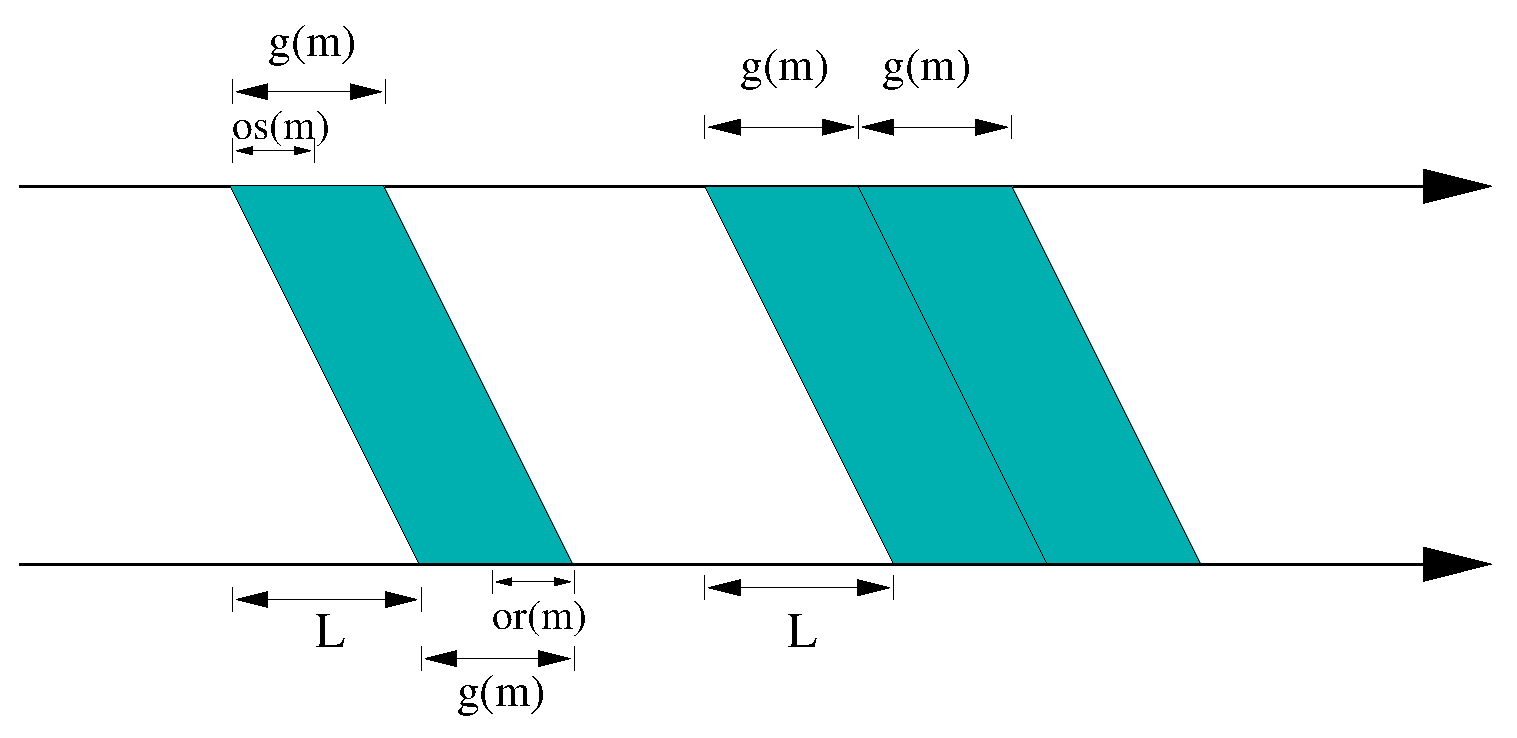
\includegraphics[width=0.7\linewidth]{images/p2p/plogp-struct}

\caption{\label{Figure: pLogP}Représentation d'une communication avec pLogP}

\end{figure}


En conséquence de cette nouvelle interprétation du \emph{gap}, les
paramètres $o_{s}$ et $o_{r}$ ont une importance moins évidente,
une fois que leur coût dans un réseau local est souvent recouvert
par celui du \textit{gap}.  Ainsi, pour représenter le temps nécessaire à la transmission d'un
message de taille \emph{m} entre deux n{\oe}uds avec des primitives de
communication bloquantes (i.e., où l'émetteur attend la fin de la transmission), le modèle pLogP utilise l'expression $L+g(m)$,
au lieu de $L+g+2o$ comme dans le modèle LogP. 


La variation des paramètres vis-à-vis de la taille des messages et des politiques d'émission est mise en évidence en Figure \ref{Figure: logp x hockney}, où on affiche les différents temps de communication mesurés avec la bibliothèque applicative LAM-MPI \cite{LAM04}. On observe un
changement de politique d'acquittement quand la taille des messages dépasse les 64 Ko, de manière à ce que le coût du \textit{gap} dépend à la fois
de la saturation de la fenêtre TCP et de la politique d'acquittement.

%
\begin{figure}
\centering
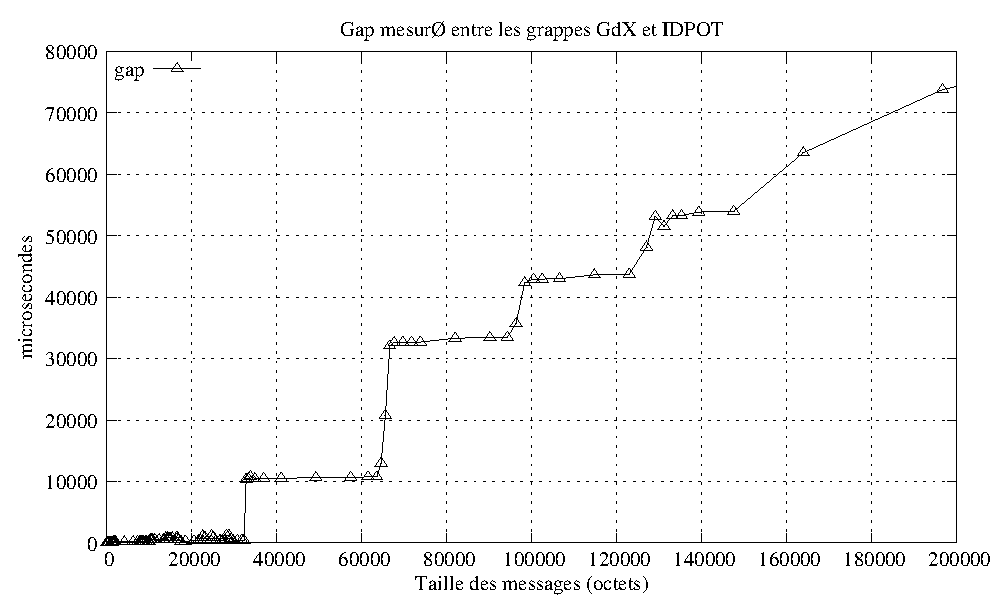
\includegraphics[width=0.7\linewidth]{images/p2p/hockney-logp1}

\caption{\label{Figure: logp x hockney}Valeurs de \textit{gap} mesurés entre deux machines
distantes \cite{Steffenel05c}}

\end{figure}



\section{Modélisation de l'Opération de Diffusion \textit{MPI\_Bcast}}

Parmi les opérations de communication collective, les diffusions de type \textit{Broadcast} sont parmi les plus simples et les plus répandues. Une opération de \emph{Broadcast} s'effectue quand un seul n{\oe}ud,
appelé \emph{racine,} envoie le même message de taille \emph{m} à
tous les autres $(P-1)$ n{\oe}uds.  Ceci représente en effet le patron de communication \textit{one-to-all}. 

Dans le cas du calcul distribué, la diffusion d'opérations est souvent nécessaire afin d'apporter des paramètres et des données à tous les n{\oe}uds.  La compréhension de ces mécanismes et la modélisation de ses coûts présente un intérêt stratégique vis-à-vis de la scalabilité et de l'optimisation des algorithmes. Dans ce sens, il est aussi nécessaire prendre en compte les différences architecturales des environnements de communication : les stratégies efficaces pour un environnement homogène diffèrent de celles adaptées aux environnements où les communications sont hétérogènes. Afin de représenter ces deux cas, nous nous sommes intéressés à la modélisation et l'optimisation des communications collectives de type \textit{Broadcast} dans deux types distincts de réseaux : les clusters (grappes de machines) et les \textit{grids} (grilles de calcul). Le premier cas  peut souvent être considéré comme homogène, alors que le deuxième apporte un degré d'hétérogénéité à cause des différences de communication intra et inter-cluster. Afin d'implémenter et valider des stratégies pour ces réseaux, nous avons choisi d'utiliser comme point de départ la bibliothèque MPI (Message Passing Interface), très utilisée par la communauté du calcul parallèle et qui dispose déjà d'une implémentation simple de l'opération \textit{broadcast} appelée MPI\_BCast.   

\subsection{\label{sec:Broadcast}Modélisation d'un \textit{Broadcast} dans un réseaux homogène}

L'opération \emph{Broadcast} est une des plus simples opérations de
communication collective : initialement, seul le n{\oe}ud \emph{racine}
détient le message qui doit être diffusé ; à la fin de l'opération,
une copie de ce message est déposée dans chaque n{\oe}ud du groupe.
L'approche classique pour implémenter l'opération \emph{Broadcast} utilise
des arbres qui sont décrits par deux paramètres, \emph{d} et \emph{h},
où \emph{d} est le nombre maximum de successeurs qu'un n{\oe}ud peut
avoir, et \emph{h} est la hauteur de cet arbre, le chemin le plus
long qui relie la racine et les feuilles de cet arbre. Plus généralement,
des arbres de diffusion avec différents degrés \emph{d} et \emph{h}
peuvent être générés à partir d'un algorithme de type \emph{arbre-alpha}
(\emph{alpha-tree} en anglais) suggéré par Bernaschi et Ianello \cite{Bernaschi98}.
À l'aide de cet algorithme et des paramètres du réseau, un arbre optimal
peut être construit à partir des paramètres du réseau et avec \emph{d,
	h $\in$}{[}1...\emph{P}-1] tel que $\sum_{i=o}^{h}d^{i}\geq P$ soit
respecté. %Cependant, pour une question de simplicité, la plupart des
%implémentations MPI utilisent des formes fixes telles que les arbres
%plats ou les arbres binomiaux. 

La performance des différentes formes fixes dépend surtout des paramètres
du réseau, notamment le \emph{gap}, la latence et le nombre de n{\oe}uds.
Par conséquent, un réseau avec une latence faible par rapport au \emph{gap}
favorise les algorithmes de type Arbre Binaire et Arbre Binomial,
qui cherchent à minimiser le temps de communication par la multiplication
des sources de transmission. Au contraire, si la latence est trop
élevée par rapport au \emph{gap}, les algorithmes de type Arbre Plat
sont favorisés, où un seul n{\oe}ud envoie des messages à tous les
autres. 


À partir des modèles de coût LogP \cite{Culler96} et pLogP \cite{Kielmann01}
et de travaux comme ceux de Huse \cite{Huse99}, Vadhiyar \cite{Vadhiyar00}
et autres, nous avons déduit les formules qui représentent différentes
stratégies de communication évaluées dans ce travail, comme indiqué
dans le Tableau \ref{table:bcast_models_classique}. Certaines de
ces stratégies sont clairement inefficaces, comme par exemple le \textit{broadcast}
en Chaîne, qui exécute $P-1$ communications en série. 

%
\begin{table}
	\centering
	\begin{tabular}{|c|c|}
		\hline 
		\textbf{\small Stratégie} & \textbf{\small Modèle de Communication}\tabularnewline
		\hline
		\hline 
		{\small Arbre Plat} & {\small $L+(P-1)\times g(m)$}\tabularnewline
		\hline 
		{\small Chaîne} & {\small $(P-1)\times(g(m)+L)$}\tabularnewline
		\hline 
		{\small Arbre Binaire} & {\small $\leq\lceil log_{2}P\rceil\times(2\times g(m)+L)$}\tabularnewline
		\hline 
		{\small Arbre Binomial} & {\small $\lceil log_{2}P\rceil\times L+\lfloor log_{2}P\rfloor\times g(m)$}\tabularnewline
		\hline
	\end{tabular}
	
	
	\caption{\label{table:bcast_models_classique}Modèles de communication pour
		le \emph{Broadcast}}
	
\end{table}


Une autre possibilité de construire un \emph{Broadcast} est la composition
des chaînes de retransmission \cite{Barnett96}. Cette stratégie,
possible grâce à la segmentation des messages, présente des avantages
importants, comme l'indiquent \cite{Kielmann01}\cite{Thakur03}\cite{Beaumont04a}.
Dans un \emph{Broadcast} Segmentée, la transmission des messages en
segments permet le recouvrement de la transmission d'un segment \emph{k}
et la réception du segment \emph{k}+1, minimisant le \emph{gap}.

Dans ce cas, nous considérons que le segment de taille \emph{s} d'un
message \emph{m} est un multiple de la taille du type basique de données
qui est transmis, divisant alors le message initial \emph{m} en \emph{k}
segments. Par conséquent, \emph{g(s)} représente le \emph{gap} d'un
segment de taille \emph{s}. Toutefois, le choix de la taille des segments
reste dépendant des caractéristiques du réseau. En effet, l'utilisation
de segments trop petits a un surcout non-négligeable dû à l'en-tête
du message, alors que l'utilisation des segments trop grands ne permet
pas l'exploitation intégrale du débit du réseau. 

La recherche de la taille de segment \emph{s} qui minimise le temps
de communication se fait à l'aide des modèles de communication présentés
dans le Tableau \ref{table:bcast_models_seg}. D'abord, on cherche
une taille de segment \emph{s} qui minimise le temps de communication
parmi $s=m/2^{i}\;\mathrm{pour}\; i\in[0\ldots log_{2}m]$. Ensuite,
on peut affiner la recherche de la taille optimale avec l'aide d'heuristiques
comme le "local hill-climbing" \cite{Kielmann01}.

%
\begin{table}
	\centering
	\begin{tabular}{|c|c|}
		\hline 
		\textbf{\small Stratégie} & \textbf{\small Modèle de Communication}\tabularnewline
		\hline
		\hline 
		{\small Arbre Plat Segmenté} & {\small $L+(P-1)\times(g(s)\times k)$}\tabularnewline
		\hline 
		{\small Chaîne Segmentée (Pipeline)} & {\small $(P-1)\times(g(s)+L)+(g(s)\times(k-1))$}\tabularnewline
		\hline 
		{\small Arbre Binomial Segmenté} & {\small $\lceil log_{2}P\rceil\times L+\lfloor log_{2}P\rfloor\times g(s)\times k$}\tabularnewline
		\hline
		{\small Pieuvre avec un degré }\emph{\small d} & {\small $(d+\lceil\frac{P-(2^{d}+1)}{(2^{d}+1)}\rceil)\times(g(s)+L)+(g(s)\times(k-1))$}\tabularnewline
		\hline
		{\small Scatter/Collection \cite{Thakur03}} & {\small $(log_{2}P+P-1)\times L+2\times(\frac{p-1}{p})\times g(m)$}\tabularnewline
		\hline
	\end{tabular}
	
	\caption{\label{table:bcast_models_seg}Modèles de communication segmentée
		pour le \emph{Broadcast}}
	
\end{table}


Pour valider ces modèles de communication, nous avons choisi la comparaison
entre les prédictions des modèles et les résultats réels obtenus à
partir d'expérimentations sur différentes plates-formes réseaux. Pour
illustrer notre approche, nous avons comparé des implémentations de
MPI\_Bcast selon les stratégies Arbre Plat, Arbre Binomial et Chaîne
Segmentée. Ainsi, les Figures \ref{Figure:Comparison-Bcast_Flat_FEth}
et \ref{Figure:Comparison-Bcast-Chain_FEth},
illustrent les valeurs mesurées expérimentalement des trois stratégies d'implémentation, qui suivent presque
fidèlement les prédictions des modèles.
%Dans les prochaines pages nous présentons l'analyse des
%expérimentations effectuées sur chaque plateforme réseau différente. 


%le réseau Fast Ethernet. 
\begin{figure}[h]
	\centering
	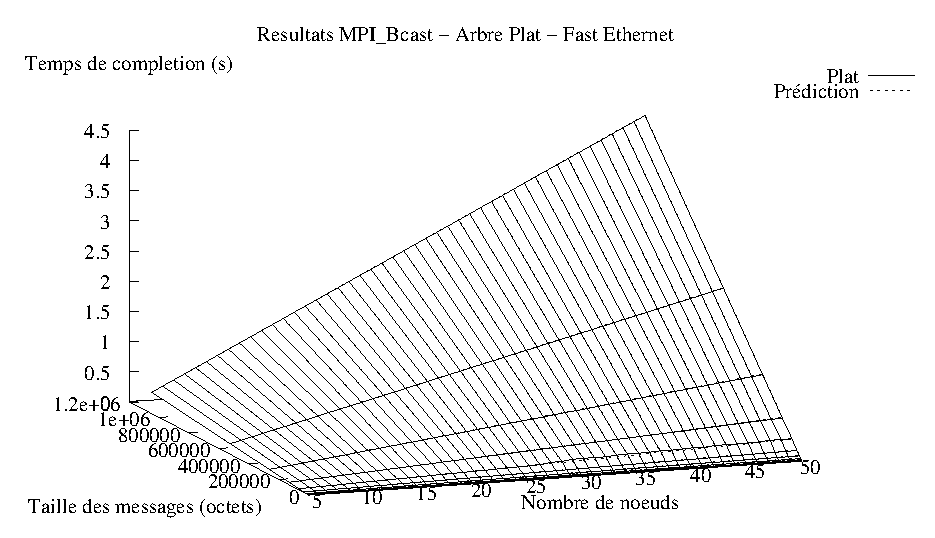
\includegraphics[width=0.5\linewidth]{images/modeles/FEth/Bcast/comp_Flat}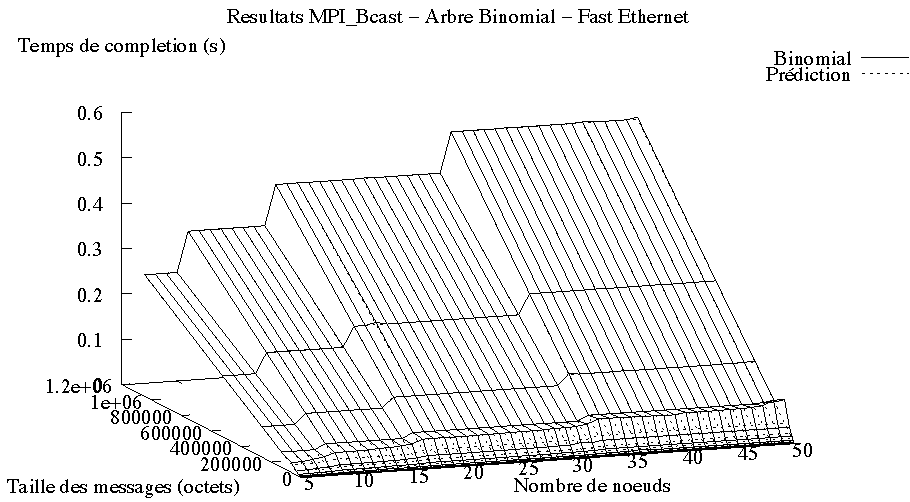
\includegraphics[width=0.5\linewidth]{images/modeles/FEth/Bcast/comp_Binomial}
	\caption{\label{Figure:Comparison-Bcast_Flat_FEth}Les performances réelles
		et prédites pour l'Arbre Plat (a) et l'Arbre Binomial (b) avec un réseau Fast Ethernet}
\end{figure}

%
\begin{figure}[h]
	\centering
	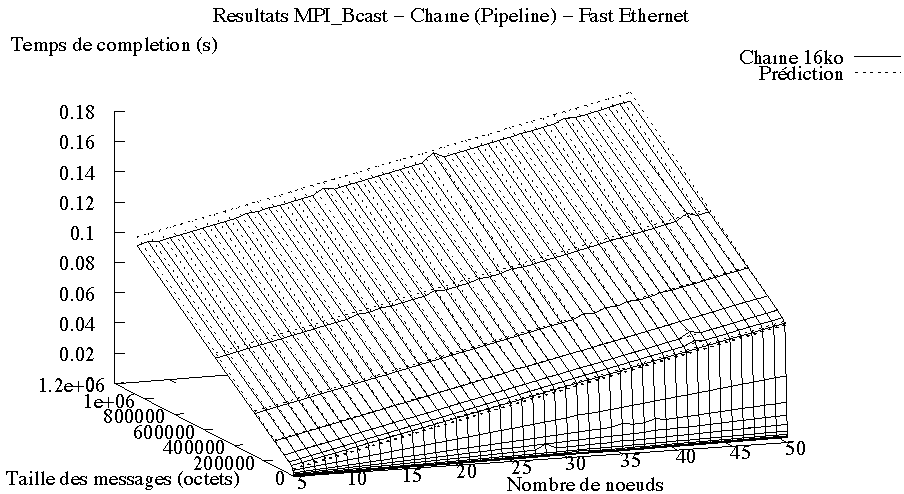
\includegraphics[width=0.5\linewidth]{images/modeles/FEth/Bcast/comp_Chain_16384}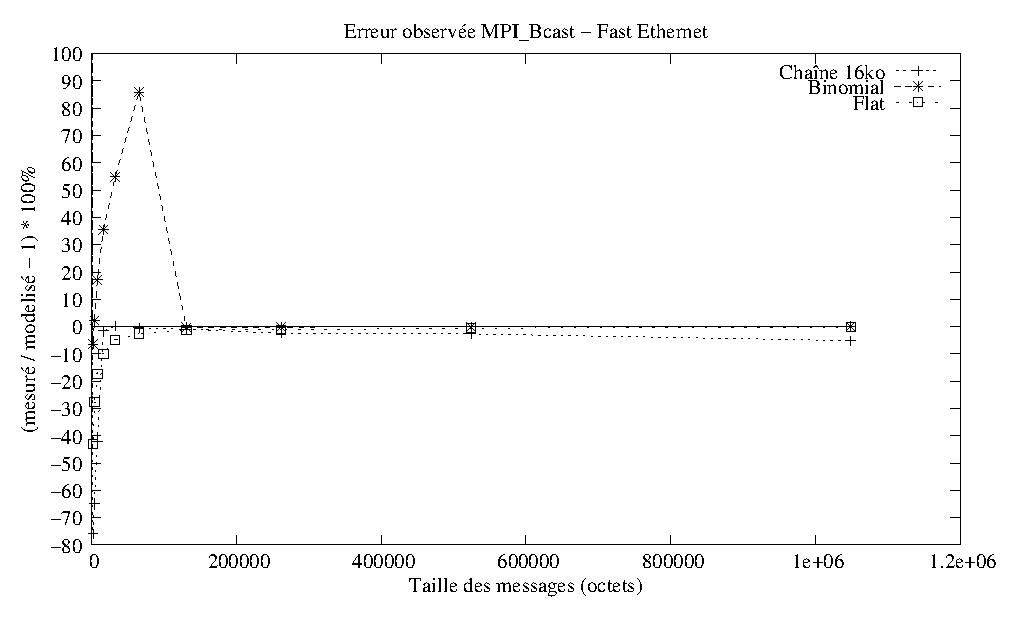
\includegraphics[width=0.5\linewidth]{images/modeles/FEth/Bcast/error}
	\caption{\label{Figure:Comparison-Bcast-Chain_FEth}Performances réelles
		et prédites pour la Chaîne Segmentée (a)  et l'erreur des prédictions par rapport
		aux valeurs mesurées (b)}
\end{figure}

Plus spécifiquement, des différences entre les prédictions et les
valeurs réelles sont observées surtout dans le cas de l'envoi de petits messages, qui ne suit pas un comportement linéaire
par rapport à la taille des messages. Cette variation de performance
a été l'objet d'analyses précédentes (cette discussion peut être retrouvée
dans les articles \cite{Steffenel04a} et \cite{Steffenel04c}) et doit son origine à l'implémentation des politiques de 
transmission et d'acquittement TCP, qui parfois opte pour retarder l'envoi de petits messages. 

En effet, TCP dispose d'une option \emph{socket} TCP\_NODELAY qui devrait permettre l'envoi de tout message sans attente. 
Seulement, nous avons observé que parfois un seul message
à chaque \emph{n} messages transmis n'est pas acquitté comme il le
faut. Cette défaillance de l'implémentation protocole d'acquittement induit un temps supplémentaire
 qui se reflète sur un surcout lors de l'envoi de petits messages.  


La Figure \ref{Figure:Comparison-Bcast-Chain_FEth} résume aussi ces trois stratégies en affichant le taux d'erreur entre les mesures et les prédictions.
Ici, nous observons que les résultats réels, normalement très proches
des prédictions (à une marge de 10\% maximum), s'écartent des prédictions
jusqu'à 90\% pour des messages autour de 128 Ko. Néanmoins, ces variations
affectent des communications où la différence absolue n'est que de
quelques millisecondes, ce qui n'empêche pas l'utilisation des modèles
de communication pour choisir la meilleure stratégie de communication. 


\subsection{Modélisation du \textit{Broadcast} dans un \textit{Grid}}

La détermination du meilleur arbre de diffusion pour un environnement
homogène est une tâche relativement facile car dépend de paramètres de latence et débit ( ou par extension, du \textit{gap}) communs à tout le réseau.  

Cependant, dans le cas d'un réseau hétérogène, ce problème devient
bien plus difficile à cause des variations des paramètres de communication entre chaque pair de n{\oe}uds. En effet, l'identification du meilleur arbre
de diffusion dans un réseau hétérogène est un problème NP-complet \cite{Bhat99}\cite{Beaumont04c,Beaumont05b}\cite{PangfengLiu04}.
La plupart des travaux dédiés à l'optimisation des communications
collectives dans des environnements hétérogènes essayent donc de construire des arbres de diffusion en tenant compte du coût d'interconnexion entre chaque pair de n{\oe}ud concernée par le \textit{broadcast}. C'est le cas de Banikazemi \cite{Banikazemi98},
Bhat \cite{Bhat99,Bhat03} ou Mateescu \cite{Mateescu05}.

Cependant, l'environnement de type \textit{grid} est normalement caractérisé
par un grand nombre de n{\oe}uds communicants, résultat de l'association
des différents \textit{clusters}. Dans ce cas, la complexité de la
tâche d'optimisation est bien plus importante, et des simplifications
s'imposent afin de permettre l'utilisation de telles méthodes dans
la pratique. Une de ces simplifications est le regroupement des n{\oe}uds
selon leurs performances relatives (par exemple, par rapport à la
communication), de manière à ce que toute une classe de n{\oe}uds
puisse être traitée comme une entité unique. De cette manière, le nombre important de n{\oe}uds dans un \textit{grid} peut être
encore facilement abordable par les méthodes d'optimisation classiques grâce à la division des communications en deux catégories, l'\textit{inter-cluster} et l'\textit{intra-cluster}. 


Cependant, à défaut de leur apport aux algorithmes de \textit{Broadcast}, ces
techniques peuvent encore être améliorées. En effet, les travaux précédents
ont été établis dans un contexte où les communications de longue distance
étaient plusieurs ordres plus lentes que celles à l'intérieur des
réseaux locaux, et la réduction des communications \textit{inter-clusters} permettait
la minimisation de la congestion sur les liens les plus lents. Si
cela est encore vrai en ce qui concerne la latence entre les n{\oe}uds,
il n'est plus exact pour le débit d'un lien de longue distance. D'autre
part, le faible coût du matériel informatique permet aujourd'hui que
les  \textit{clusters} regroupent des centaines de n{\oe}uds. Or, plus le coût de
diffusion \textit{intra-clusters} devient important, plus son influence
sur la performance sera importante au moment de définir l'ordonnancement
des communications.

C'est exactement ce qui différencie les heuristiques traitant (ou
ne traitant pas) la communication à l'intérieur des groupes : les
heuristiques "traditionnelles" et celle appelées "heuristiques
sensibles au contexte des \textit{grids}" ("\emph{grid-aware}"
en anglais). Dans le premier cas, l'optimisation ne tient compte que
des communications entre les différents coordinateurs, alors que le
deuxième cas s'occupe aussi de la diffusion à l'intérieur des  \textit{clusters}. 


Les prochaines sections présentent les différentes heuristiques étudiées
pour l'optimisation des communications de type MPI\_Bcast. Certaines
de ces heuristiques sont la simple application des méthodes pour les
réseaux hétérogènes dans le contexte des  \textit{clusters} hiérarchisées. Dans
ce travail nous proposons trois nouvelles méthodes, qui au contraire
des techniques précédentes, considèrent autant les communications
entre les coordinateurs que les temps nécessaires à la diffusion des
messages à l'intérieur des  \textit{clusters}.


\subsubsection*{Formalisme utilisé}

Pour décrire les heuristiques présentées dans cette section, nous
utilisons un formalisme de groupes similaire à celui de Bhat \cite{Bhat03}.
Dans ce formalisme, les  \textit{clusters} sont séparés en deux groupes, \textbf{A}
et \textbf{B}. Le groupe \textbf{A} contient les  \textit{clusters} qui ont déjà
reçu le message (la réception du message par le coordinateur du
 \textit{cluster} est suffisante). Le groupe \textbf{B} contient les  \textit{clusters}
qui devront recevoir le message. De cette manière, le groupe \textbf{A}
contient initialement le  \textit{cluster} du n{\oe}ud \emph{source} ou \emph{racine},
tandis que le groupe \textbf{B} contient toutes les autres  \textit{clusters}
du réseau.

À chaque étape, un émetteur appartenant au groupe \textbf{A} et un
récepteur appartenant au groupe \textbf{B} sont choisis. Après la
communication entre ces deux  \textit{clusters} (plus exactement, leurs coordinateurs),
le \textit{cluster} récepteur est transféré au groupe \textbf{A}. 

L'implémentation de ces communications est faite de manière à rendre
prioritaires les communications entre les  \textit{clusters}. En effet, les coordinateurs
diffusent le message à l'intérieur de ses  \textit{clusters} seulement après
la fin des communications \textit{inter-clusters}. Cette stratégie favorise
la multiplication des sources disponibles et l'application des heuristiques,
ainsi que la prédiction du temps total d'exécution du \textit{Broadcast}.

\subsubsection{Heuristiques Traditionnelles}

\subsubsection*{Diffusion en Arbre Plat (Flat)}

L'heuristique en \emph{Arbre Plat}, découpe la communication en deux niveaux, \emph{inter-clusters}
et \emph{intra-clusters}. 

Dans le premier niveau, le n{\oe}ud \emph{racine} envoie le message
à tous les coordinateurs des différents \textit{clusters}. L'ordre d'envoi
suit le "rang" des différents \textit{clusters}, prédéfini à l'initialisation.
Formellement, cela veut dire qu'à chaque étape, le n{\oe}ud \emph{racine}
choisi comme récepteur le premier  \textit{cluster} du groupe \textbf{B}. Dans
cette "heuristique", le n{\oe}ud émetteur est toujours
le même (le n{\oe}ud \emph{racine}), malgré le fait que les  \textit{clusters}
qui ont déjà reçu le message font désormais partie du groupe \textbf{A}.
Dans le deuxième niveau de diffusion, exécuté à l'intérieur de chaque
 \textit{cluster}, les coordinateurs exécutent un \emph{broadcast} en arbre binomial.

Même si cette heuristique est très simple à implémenter, elle est toutefois
très peu optimisée. En effet, la diffusion des données ne tient pas
compte des performances des différents  \textit{clusters}, ni les vitesses d'interconnexion
entre les \emph{coordinateurs}. Même si l'utilisateur organise le
fichier de description des  \textit{clusters} de manière à favoriser les communications
émises d'un certain  \textit{cluster}, celles-ci restent soumises à une structure
de diffusion \emph{plate}. 


\subsubsection*{Fastest Node First - FNF}

L'heuristique \emph{Fastest Node First} (le n{\oe}ud le plus rapide d'abord)
a été proposée par Banikazemi \emph{et al.} \cite{Banikazemi98}.
Dans leur modèle de communication, le réseau est composé d'un certain
nombre de n{\oe}uds \emph{$P$}. À chaque n{\oe}ud \emph{$P_{\textrm{i}}$}
on associe un coût d'envoi \emph{$C_{\textrm{i}}$}. Ce coût \emph{$C_{\textrm{i}}$}
est indépendant de la destination et de la taille du message, et indique
seulement la différence de vitesse entre les n{\oe}uds.

L'heuristique proposée par Banikazemi \emph{et al.} nécessite $P-1$
itérations, où à chaque étape l'heuristique définie un émetteur et
un récepteur. Le récepteur est choisi parmi les possibles récepteurs
du groupe \textbf{B} dont le coût \emph{$C_{\textrm{i}}$} est le
plus petit. L'émetteur est le n{\oe}ud du groupe \textbf{A} qui peut
finir la communication le plus rapidement possible. Cela dit, cette
stratégie choisit l'émetteur le plus rapide et le récepteur qui pourrait
retransmettre les messages le plus rapidement possible, à son tour.

L'efficacité de l'heuristique FNF dans le cadre des environnements
homogènes a été démontrée par Liu \cite{PangfengLiu00b}, qui a prouvé que
l'heuristique FNF produit des ordonnancements avec au plus deux fois
le temps optimal.

Cependant, des environnements homogènes comme ceux considérés par
Banikazemi sont assez rares dans les \textit{grids}, ce qui rend cette heuristique
très limitée par rapport à la modélisation des communications. En
effet, le modèle de coût unique $C_{\textrm{i}}$ n'est pas suffisant
pour représenter l'hétérogénéité d'un réseau d'interconnexion, comme
indiqué par Bhat \cite{Bhat03}. 


\subsubsection*{Fastest Edge First - FEF}

Proposée par Bhat \emph{et al.} \cite{Bhat03}, l'heuristique \emph{Fastest
	Edge First} (l'arête la plus rapide d'abord) est un algorithme glouton
qui fait partie d'une collection d'heuristiques proposées comme alternative
à l'heuristique FNF. 

Assez simple, cette heuristique est très similaire à l'heuristique
FNF. Seulement, au lieu d'un coût de communication unique $C_{\textrm{i}}$,
l'heuristique évalue le poids de chaque lien de communication $L_{i,j}$
entre deux n{\oe}uds différents (les arêtes), correspondants à la latence
de communication entre les deux n{\oe}uds. 

Pour identifier l'ordonnancement des communications nécessaire à l'exécution
de l'opération de \textit{Broadcast}, l'algorithme FEF, ordonne les n{\oe}uds
du groupe A selon leurs arêtes les plus rapides. Cela permet le choix
du lien le plus rapide parmi toutes les possibilités, et en même temps,
sert à définir l'émetteur et le récepteur, déterminés implicitement
par l'arête choisie. Une fois que le récepteur est désigné, celui-ci
est transféré du groupe \textbf{B} vers le groupe \textbf{A}. À cet
instant, les arêtes minimales doivent être recalculées.

Le raisonnement de cette heuristique est que le choix des liens les
plus rapides permet d'augmenter rapidement le nombre d'émetteurs.
À leur tour, ces émetteurs pourront disséminer le message vers les
n{\oe}uds les plus éloignés, tout en choisissant le lien le moins
coûteux.


\subsubsection*{Early Completion Edge First - ECEF}

Selon les heuristiques précédentes, une fois que le récepteur était
assigné, celui-ci était immédiatement transféré vers le groupe des
émetteurs, le groupe \textbf{A}. Toutefois, à cause des délais de
communication, il est possible que ce récepteur n'ait pas encore reçu
le message et qu'il soit choisi pour le retransmettre à un deuxième
n{\oe}ud. La communication subira un retard supplémentaire, alors
qu'une autre arête, moins rapide, pourrait finir la transmission plus
vite si son émetteur a déjà le message. 

Pour tenir compte des retards dus à la transmission des données, l'heuristique
\emph{Early Completion Edge First} (arête qui finit le plus tôt) considère
aussi dans son évaluation l'instant où les émetteurs ont les données
disponibles pour l'envoi. Ainsi, la \emph{disponibilité} $RT_{i}$
du n{\oe}ud émetteur (\emph{Ready Time} en anglais) est alors utilisée
conjointement avec le temps nécessaire à la transmission du message
entre les n{\oe}uds (le \textit{gap} plus la latence) de manière à choisir
le couple émetteur-récepteur qui minimise le temps : 

\[
RT_{i}+g_{i,j}(m)+L_{i,j}\]


Ainsi, l'objectif de cette heuristique est d'augmenter le nombre de
n{\oe}uds qui peuvent \emph{effectivement} transmettre les messages
aux autres n{\oe}uds.


\subsubsection*{Early Completion Edge First with lookahead - ECEF-LA}

Pour augmenter l'efficacité de l'heuristique précédente, la dernière
heuristique proposée par Bhat \emph{et al.} \cite{Bhat03} propose
une recherche plus approfondie sur les possibles choix. En effet,
si l'objectif des heuristiques précédentes était la multiplication
des sources disponibles, cela suppose que ces sources pourront, à
leur tour, retransmettre les messages de manière efficace.

C'est ainsi que Bhat a proposé l'utilisation d'une fonction de \emph{lookahead}
(recherche en avant) pour évaluer si le choix d'un récepteur est réellement
bon. De cette manière, l'algorithme calcule préalablement la fonction
de \emph{lookahead} $F_{j}$ pour tous les n{\oe}uds dans le groupe
\textbf{B}, et la pair émetteur-récepteur est celle qui minimise
la somme :

\[
RT_{i}+g_{i,j}(m)+L_{i,j}+F_{j}\]


Cette fonction de \emph{lookahead} peut être définie de plusieurs
façons. Bhat \cite{Bhat03} propose, par exemple, le coût minimal
pour que le n{\oe}ud \emph{j} transmette à d'autres n{\oe}uds encore
dans le groupe \textbf{B}. Cette fonction est alors la suivante :

\begin{eqnarray*}
	F_{j} & = & \min_{P_{k}\in B}\,(g_{j,k}(m)+L_{j,k})\end{eqnarray*}


Intuitivement, cette fonction indique l'utilité du n{\oe}ud $P_{j}$
si à son tour il est transféré vers le groupe \textbf{A}. D'ailleurs,
Bhat a proposé d'autres fonctions de \emph{lookahead}, dont par exemple
la moyenne de la latence entre $P_{j}$ et les autres n{\oe}uds en
\textbf{B}, ou alors la latence moyenne entre les émetteurs et les
récepteurs, si on considère que $P_{j}$ est transféré vers le groupe
\textbf{A}. 


\subsubsection{Heuristiques "grid-aware"}

Les heuristiques présentées précédemment hiérarchisent les communications en deux niveaux - \emph{inter-clusters}
et \emph{intra-clusters}, mais les fonctions d'évaluation ne tiennent compte que des coûts de transmission entre les coordinateurs
des différentes  \textit{clusters} du réseau.

Comme nous l'avons déjà exposé, le coût d'une communication
hiérarchique ne dépend pas seulement des latences entre les différentes
 \textit{clusters}, mais aussi du temps nécessaire à la diffusion des messages
à l'intérieur de ces  \textit{clusters}. Ce coût de diffusion \textit{intra-clusters} devient
encore plus important avec l'augmentation du nombre de n{\oe}uds à l'intérieur
des  \textit{clusters}, qui aujourd'hui dépasse facilement la centaine de machines.
Par exemple, l'envoi d'un message de 1Mo entre deux \textit{clusters} (l'un à Grenoble, l'autre à Paris) requiert 349 millisecondes, alors que
le \textit{broadcast} de ce même message entre 50 n{\oe}uds du \textit{cluster} de Grenoble
peut nécessiter jusqu'à 3 secondes selon l'algorithme
utilisé. Si ce temps n'est pas pris en compte lors de la modélisation
des communications, l'ordonnancement des communications risque d'être
sous-optimal.

Plus exactement, le temps de diffusion \textit{intra-clusters}, appelé $T_{k}$,
correspond aux prédictions des modèles de communication vus précédemment. 
Cette notation $T_{k}$ est équivalente à une notation où un n{\oe}ud
fictif $k'$ est associé à chaque coordinateur $k$, dont :

\[
L_{k,k'}+g_{k,k'}=\left\{ \begin{array}{c}
\begin{array}{cc}
T_{k} & si\: k'\, est\, associe\, a\, k\\
\infty & \,\,\,\,\,\,\,\,\,\,\,\,\, pour\, tout\, autre\, noeud\, j\neq k\end{array}\end{array}\right.\]


La présence d'un n{\oe}ud fictif permet l'utilisation des heuristiques
précédentes sans la nécessité d'une modification des algorithmes,
notamment le ECEF. L'utilisation de $T_{k}$ permet une implémentation
plus simple des algorithmes, qui n'ont pas besoin de garder les deux
identités \emph{k} et \emph{k'} associées à un  \textit{cluster} \emph{k}. Toutefois, dans ce travail nous avons gardé
la description séparée \emph{L}, \emph{g} et \emph{T}, afin
de permettre une identification plus facile des facteurs évalués.

Dans ce sens, nous présentons deux nouvelles stratégies d'évaluation
dites "sensibles au contexte des \textit{grids}", où
le temps de diffusion \emph{intra-cluster} est aussi considéré lors
de la construction des arbres de diffusion. Pour mieux analyser l'efficacité
de ces stratégies, nous avons aussi développé une version de l'heuristique
ECEF-LA où le temps \textit{intra-clusters} est pris en compte. Cette version
sert de comparaison par rapport aux heuristiques de Bhat, présentées
précédemment. 


\subsubsection*{ECEF-LA\emph{t}}

L'heuristique ECEF-LA\emph{t} est l'évolution naturelle de l'heuristique
ECEF-LA où nous utilisons une fonction de \emph{lookahead} adaptée
à la représentation du coût de communication \textit{intra-clusters} $T_{k}$. 

Ainsi, l'heuristique ECEF-LA\emph{t} cherche à minimiser le coût total
de transmission et le temps nécessaire à la diffusion d'un message
dans un  \textit{cluster} distant (en effet, le "petit \emph{t}"
du nom de cette heuristique indique qu'on cherche le minimum des temps).
Pour cela, elle utilise une fonction d'évaluation :

\begin{eqnarray*}
	F_{j} & = & \min_{P_{k}\in B}\,(g_{j,k}(m)+L_{j,k}+T_{k})\end{eqnarray*}


À l'instar de l'heuristique ECEF-LA, le but de cette stratégie est
que le récepteur soit choisi parmi les  \textit{clusters} qui peuvent retransmettre
le message le plus vite possible à d'autres  \textit{clusters}. L'adjonction
du temps $T_{k}$ dans la fonction d'évaluation implique aussi que
le choix d'un interlocuteur minimisera le temps de complétion des
 \textit{clusters} contactés dans le futur. 


\subsubsection*{ECEF-LA\emph{T}}

Une contrepartie de la technique précédente est que cette stratégie
a tendance à favoriser les  \textit{clusters} rapides, ce qui peut entraîner
des retards supplémentaires aux  \textit{clusters} plus lents, reléguées aux
dernières places. Pour éviter une telle situation, nous proposons
une nouvelle fonction de \emph{lookahead}, où le choix des  \textit{clusters}
considère le maximum du temps nécessaire à la transmission et à la
diffusion d'un message : 

\begin{eqnarray*}
	F_{j} & = & \max_{P_{k}\in B}\,(g_{j,k}(m)+L_{j,k}+T_{k})\end{eqnarray*}


Malgré sa similarité avec l'heuristique précédente, cette nouvelle
fonction d'évaluation cherche à équilibrer le temps de communication
vers les différents  \textit{clusters}, lentes ou rapides. En effet, nous cherchons
dans un premier instant le  \textit{cluster} la plus lente qu'il reste à contacter
(la fonction de \emph{lookahead}), et parmi les choix d'émetteurs
disponibles, nous choisissons celui qui peut la contacter le plus
rapidement possible (fonction d'évaluation \emph{min} de l'heuristique
ECEF).

Le raisonnement de cette heuristique est que si les  \textit{clusters} les plus
distants ou les plus lents (dans le sens où la diffusion des messages
prend plus de temps) sont contactés en dernière place, leur diffusion
prendra encore plus de retard, ce qui augmentera le temps d'exécution
du \textit{Broadcast}. Avec la fonction de \emph{lookahead} de ECEF-LA\emph{T},
nous choisissons comme récepteur le  \textit{cluster} qui prendra le moins de
temps possible pour contacter le  \textit{cluster} le plus lent : cela garantit
que si besoin est, les  \textit{clusters} les plus lents seront contactés dans
le minimum de temps possible.


\subsubsection*{BottomUp}

La troisième heuristique proposée dans ce travail utilise une logique
d'optimisation différente de celle utilisée par Bhat. En effet, l'approche
de Bhat vise toujours la minimisation des facteurs liés à la transmission
des messages et à sa diffusion, ce qui généralement finit par donner
priorité aux  \textit{clusters} les plus rapides. Cependant, nous considérons
que le temps d'exécution d'un \textit{Broadcast} hiérarchique dépend surtout
des  \textit{clusters} les plus lents.

À partir des heuristiques précédentes, nous observons que, malgré
l'utilisation de différentes fonctions de \emph{lookahead}, les heuristiques
de type ECEF-LA suivent toujours l'approche \emph{min-max} ou \emph{min-min}.
Or, l'heuristique ECEF-LA\emph{T} considère que parfois il est plus
intéressant d'envoyer les messages d'abord aux  \textit{clusters} les plus lents,
pour ne pas retarder encore plus leur diffusion. D'autre part, il
est aussi vrai qu'un grand nombre d'émetteurs favorise la conclusion
rapide du \textit{Broadcast}, et que l'envoi à des  \textit{clusters} plus lents n'aide
guère à augmenter le nombre d'émetteurs. Si ces deux raisonnements
sont a priori opposés, ils ne sont pas incompatibles. En effet, les
deux approches peuvent être combinées si des règles précises sont
déterminées.

C'est ainsi que dans l'heuristique \textit{BottomUp} nous définissons initialement
une approche de type \emph{max-min}, où l'émetteur est choisi parmi
les  \textit{clusters} qui pourront contacter le plus rapidement possible le
 \textit{cluster} le plus lent du réseau :

\[
\max_{P_{j}\in B}\,(\min_{P_{i}\in A}\,(g_{i,j}(m)+L_{i,j}+T_{j}))\]


En effet, cette approche permet que les  \textit{clusters} les plus lents soient
contactés dans le plus petit temps possible, ce qui peut minimiser
le retard imputé à ces  \textit{clusters}. Toutefois, cette technique n'offre
aucune garantie sur l'efficacité future des  \textit{clusters} émetteurs. Pour
cela, il serait peut-être intéressant d'ajouter une fonction de \emph{lookahead},
à l'exemple des heuristiques de type ECEF-LA.


\subsection{Évaluation pratique}

Les différentes heuristiques ont été implémentées sur une version modifiée
de la bibliothèque MagPIe\cite{Kielmann99b}, que nous avons adapté pour l'acquisition
et la manipulation des paramètres de communication entre les  \textit{clusters}. Cette procédure de
découverte de topologie permet non seulement le regroupement des n{\oe}uds
en \textit{clusters} logiques homogènes (plus adaptées à la modélisation de
performance), mais aussi fait automatiquement l'acquisition des paramètres
pLogP correspondant à chaque sous-réseau homogène. Ces paramètres
pLogP, une fois chargés en mémoire, sont associés à la structure hiérarchique
du réseau. Ils sont utilisés pour prédire la performance des communications et pour choisir les meilleures
stratégies selon les caractéristiques des réseaux.

Pour cette validation nous avons utilisé 88 machines réparties entre les \textit{clusters}
d'Orsay, Toulouse et Grenoble. Nous avons utilisé 60 machines
du  \textit{cluster} d'Orsay, 20 machines du  \textit{cluster} de Toulouse et
8 machines du  \textit{cluster} de Grenoble. Après la découverte de la topologie du réseau, ces machines ont été regroupées en 6
\textit{clusters} homogènes différentes comme indiqué par le Tableau \ref{Tableau: Latence grid 1}. 

\begin{table}
	\caption{\label{Tableau: Latence grid 1}Latence entre les différents \textit{clusters}
		(en microsecondes)}
	
	
	\begin{centering}
		{\footnotesize }\begin{tabular}{|c||c|c|c|c|c|c|}
			\hline 
			& {\footnotesize  Cluster 0} & {\footnotesize  Cluster 1} & {\footnotesize  Cluster 2} & {\footnotesize Cluster 3} & {\footnotesize  Cluster 4} & {\footnotesize  Cluster 5}\tabularnewline
			\hline 
			& {\footnotesize 31 x Orsay} & {\footnotesize 29 x Orsay} & {\footnotesize 6 x IDPOT} & {\footnotesize 1 x IDPOT} & {\footnotesize 1 x IDPOT} & {\footnotesize 20 x Toulouse}\tabularnewline
			\hline
			\hline 
			{\footnotesize  Cluster 0} & {\footnotesize 47.56} & {\footnotesize 62.10} & {\footnotesize 12181.52} & {\footnotesize 12187.24} & {\footnotesize 12197.49} & {\footnotesize 5210.99}\tabularnewline
			\hline 
			{\footnotesize  Cluster 1} & {\footnotesize 62.10} & {\footnotesize 47.92} & {\footnotesize 12181.52} & {\footnotesize 12198.03} & {\footnotesize 12195.22} & {\footnotesize 5211.47}\tabularnewline
			\hline 
			{\footnotesize  Cluster 2} & {\footnotesize 12181.52} & {\footnotesize 12181.52} & {\footnotesize 35.52} & {\footnotesize 60.08} & {\footnotesize 60.08} & {\footnotesize 5388.49}\tabularnewline
			\hline 
			{\footnotesize  Cluster 3} & {\footnotesize 12187.24} & {\footnotesize 12198.03} & {\footnotesize 60.08} & {\footnotesize 0$^{*}$} & {\footnotesize 242.47} & {\footnotesize 5393.98}\tabularnewline
			\hline 
			{\footnotesize  Cluster 4} & {\footnotesize 12197.49} & {\footnotesize 12195.22} & {\footnotesize 60.08} & {\footnotesize 242.47} & {\footnotesize 0$^{*}$} & {\footnotesize 5394.10}\tabularnewline
			\hline 
			{\footnotesize  Cluster 5} & {\footnotesize 5210.99} & {\footnotesize 5211.47} & {\footnotesize 5388.49} & {\footnotesize 5393.98} & {\footnotesize 5394.10} & {\footnotesize 27.53}\tabularnewline
			\hline
		\end{tabular}
		\par\end{centering}{\footnotesize \par}
	
	\begin{centering}
		{\footnotesize {*} ce \textit{cluster} contient une seule machine.}
		\par\end{centering}
\end{table}


La Figure \ref{Figure: Bcast - Case1 - Mesure} présente ainsi les temps de communication de chacune de ces stratégies. Le premier résultat à noter est la faible performance de la stratégie
\textit{Flat}, même par rapport à l'implémentation par défaut de MPI. Cela
ne veut pas dire que la stratégie \textit{Flat} est toujours moins performante
que les autres stratégies, mais indique que cette stratégie est trop
dépendante de la configuration du réseau, de l'ordre de représentation
des \textit{clusters} et du n{\oe}ud racine.
%
\begin{figure}[h]
	\centering
		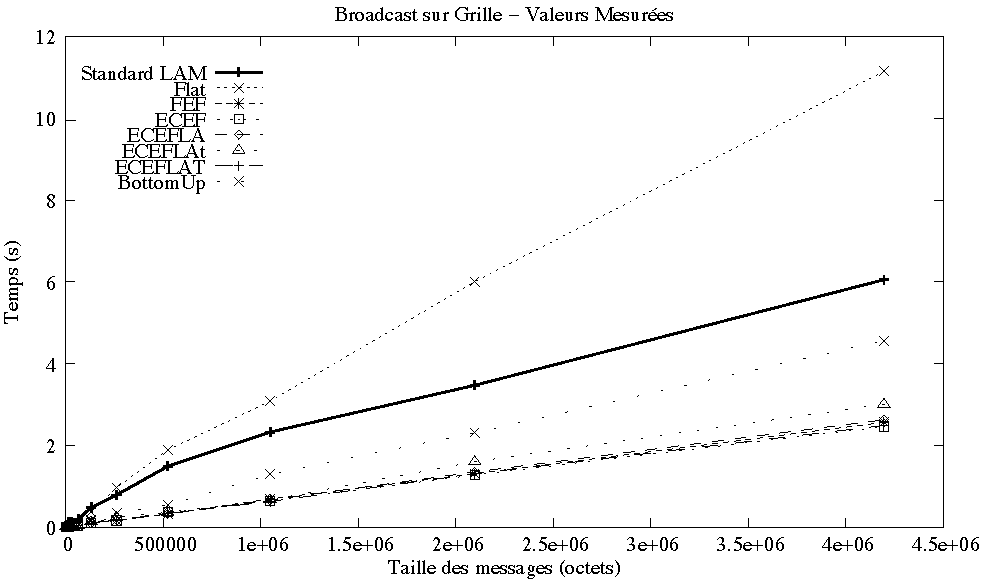
\includegraphics[width=0.7\linewidth]{images/Grid/Bcast/case1/comp}
	\caption{\label{Figure: Bcast - Case1 - Mesure}Performance du \textit{Broadcast} sur
		un \textit{grid} de 88 machines }	
\end{figure}

\begin{figure}[h]
	\centering
		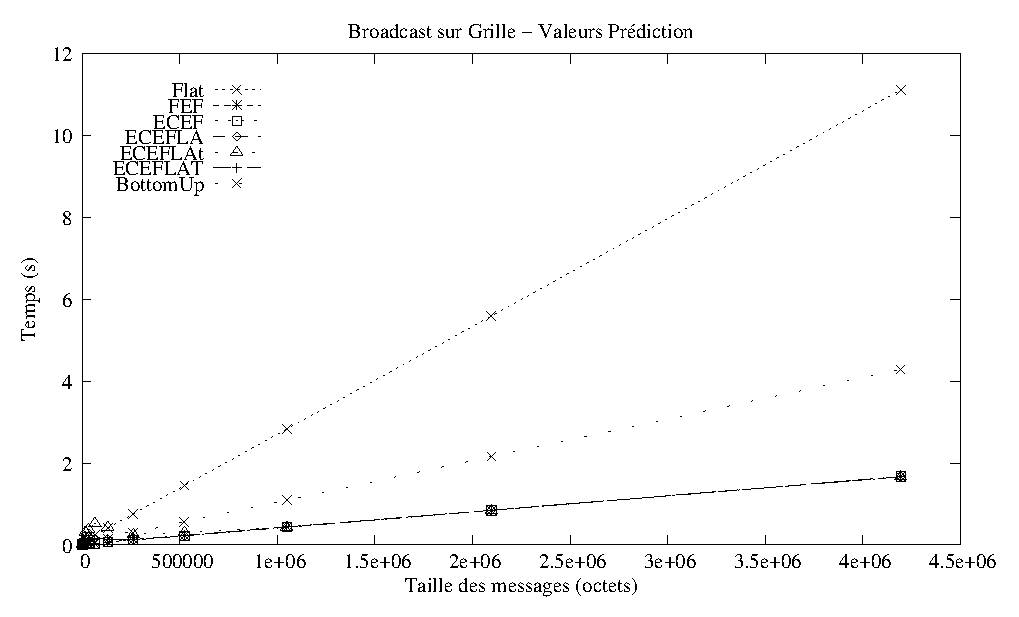
\includegraphics[width=0.7\linewidth]{images/Grid/Bcast/case1/simul}	
	\caption{\label{Figure: Bcastcase1predictions}Prédictions pour un \textit{grid}
		avec 88 machines}
	
\end{figure}

Dans le cas des autres heuristiques, on observe des gains de performance
déjà très importants. L'heuristique \textit{BottomUp} %, comme prévu par lessimulations, 
n'est pas aussi efficace que les autres heuristiques,
qui de leur côté, se comportent de manière très similaire.

Le faible écart observé entre les prédictions des heuristiques de
type FEF et ECEF-{*} est justifié surtout par le nombre réduit de
\textit{clusters}, qui réduit le nombre de combinaisons possibles et fait converger
les résultats des différentes heuristiques. 

Pour mieux valider les résultats des expériences, la Figure \ref{Figure: Bcastcase1predictions}
présente les temps prévus des différentes heuristiques. Ces temps,
calculés automatiquement par les heuristiques d'ordonnancement des
communications, donnent une meilleure indication de la fiabilité des
modèles par rapport aux résultats pratiques. Dans ce cas, nous observons
que les heuristiques de type FEF et ECEF-{*} ont des résultats très
rapprochés, certainement parce qu'elles ont obtenu le même ordonnancement
des communications. D'un autre côté, l'écart entre ces prédictions
et les résultats réels sont bien plus importants pour les heuristiques
FEF et ECEF-{*} que pour le \textit{BottomUp} ou le \textit{Flat}. Cela indique que
le coût du calcul de l'ordonnancement et le coût de la mise en {\oe}uvre
de ces communications sont les facteurs les plus importants, et reflètent
l'augmentation de complexité d'une communication à couches multiples.

Cette étude met en évidence l'importance
du n{\oe}ud racine et de la répartition des n{\oe}uds sur des différents
\textit{clusters} sur la performance des stratégies plus simples. En effet,
la performance de la stratégie \textit{Flat} est fortement liée à l'ordre des \textit{clusters}, généralement fournie par l'utilisateur.
De surcroît, la stratégie \textit{Flat} utilise toujours le même ordre de diffusion,
indépendamment du rang du n{\oe}ud racine. Au contraire, les heuristiques
les plus élaborées construisent des arbres de diffusion adaptés à
chaque situation, ce qui rend possible un gain de performance plus
important, surtout quand le rôle de \emph{racine} est alterné entre
plusieurs n{\oe}uds.

D'ailleurs, les simulations indiquent que la performance des stratégies
simples, comme le \textit{Flat}, supportent très mal l'augmentation du nombre
de \textit{clusters} interconnectés.  Ainsi, nous croyons que, même si
le \textit{grid} compte un nombre réduit de \textit{clusters}, l'utilisation d'une
heuristique un peu plus élaborée, comme par exemple l'heuristique
ECEFLA-T, offre le meilleur rapport coût-bénéfice-robustesse.


\section{Amélioration de la Performance de MPI\_AlltoAll dans un \textit{Grid}}

Si les stratégies présentées dans les sections précédentes permettent l'optimisation des communications dans le cadre d'une diffusion MPI\_Bcast, d'autres patrons de communication encore plus couteux sont utilisés par les applications scientifiques. L'une de ces patrons, le \textit{many-to-many}, représente un \emph{échange total} d'informations entre les n{\oe}uds \cite{Christara99}. Plus exactement, chaque n{\oe}ud détient $n$ items de données différentes de taille $m$, lesquels doivent être distribués entre $n$ n{\oe}uds (le n{\oe}ud inclus).  

Vu la complexité de l'opération, les implémentations de \textit{many-to-many} dans la bibliothèque MPI (appelées "\textit{All-to-All}" par celle-ci) généralement utilisent des envois directs entre les n{\oe}uds, ce qui peut occasionner la surcharge des communications et des problèmes liés à la congestion du réseau. De surcroît, l'utilisation de cette approche dans un environnement de type grille doit aussi faire face à l'hétérogénéité des temps de communication entre les n{\oe}uds proches et distants.

\subsection{Définitions}

Soit deux \textit{clusters} ${\mathcal C}_1$
et ${\mathcal C}_2$ avec respectivement $n_1$ n{\oe}uds et $n_2$ n{\oe}uds.
Un réseau, appelé \textit{backbone}, interconnecte les deux \textit{clusters}. Nous assumons aussi que l'interface réseau utilisée pour la communication avec un réseau distant est la même utilisée pour la communication avec le réseau local. De ce fait et de la topologie du réseau, les communications \textit{inter-cluster} ne seront jamais plus rapides que celles effectuées à l'intérieur d'un \textit{cluster}.

Maintenant supposons qu'une application doit échanger des données entre les machines dans ${\mathcal C}_1$ et ${\mathcal C}_2$ et que pour chaque source, les données à destination des autres machines ne sont pas identiques (mais ont toutes une taille $m$).  Comme résultat, nous devons transmettre l'équivalent à $(n_1+ n_2)^2$ messages différents. Alors que plusieurs bibliothèques MPI  (OpenMPI, MPICH2, etc.) implémentent l'opération \textit{MPI\_AllltoAll} en supposant que les n{\oe}uds se trouvent dans le même réseau et donc que les communications ont le même coût, dans notre cas certains messages sont envoyés entre n{\oe}uds d'un même \textit{cluster} et d'autres entre n{\oe}uds de réseaux différents. Dans le premier cas, la latence des communications est plus favorable que dans le deuxième, et souvent le même principe s'applique pour le débit du réseau.


\subsection{Modélisation de la Congestion du Réseau\label{cluster}}

La communication intensive engendrée par les opérations de type \textit{alltoall} peut facilement saturer le réseau ou les destinataires, dégradant ainsi la performance globale de l'opération. Chun \cite{Chun01} a démontré que le coût des communications collectives est souvent dominé par le coût de la congestion du réseau et des subséquentes pertes de paquets.

Malheureusement, plusieurs modèles de communication tels que \cite{Christara99} ou \cite{Pjesivac-Grbovic05} ne prennent pas en compte les impacts potentiels de la congestion. En effet, ces travaux considèrent que l'opération All-to-All n'est qu'une exécution parallèle de plusieurs opérations de type \emph{personalized one-to-many} \cite{Johnsson89}. Cela s'exprime par le modèle de performances linéaire représenté en Equation \ref{eq:1}, où $\alpha$ correspond à la latence de communication entre les n{\oe}uds, $\frac{1}{\beta}$ correspond au débit du lien, $m$ représente la taille des messages en octets et  $n$ correspond au nombre de n{\oe}uds :
\begin{equation}
T=(n-1)\times(\alpha+\beta m)\label{eq:1}
\end{equation}

Comme ce modèle linéaire n'est pas capable de prendre en compte la congestion des communications, certains auteurs tels que Bruck \cite{Bruck97b} et Clement \emph{et al.} \cite{Clement96} suggèrent l'utilisation d'un facteur de ralentissement (\emph{slowdown factor}) proportionnel au nombre de n{\oe}uds communicants.  Labarta et \emph{al.} \cite{Labarta96} aussi suggère l'utilisation d'un facteur de ralentissement basé sur le nombre de messages en transit car, selon eux, si \emph{m} messages sont prêts à être transmis mais seulement \emph{b} canaux sont disponibles, alors les transmissions sont sérialisées en $\left\lceil \frac{m}{b}\right\rceil $ vagues de communication. 

Une approche légèrement différente a été proposée par Chun \cite{Chun01}, qui associe la congestion à la latence et donc utilise différentes valeurs de latence selon la taille des messages. Cependant, ce modèle ignore le nombre de messages circulant sur un réseau ou un lien, alors et ceci est directement lié au phénomène de la congestion. 

Afin de mieux représenter l'impact de la congestion sur les communications collectives de type All-to-All dans les \textit{clusters}, nous avons proposé en \cite{Steffenel06b} un modèle où la congestion du réseau est dépendant des caractéristiques de l'environnement physique (interfaces réseaux, liens, switches) mais aussi de la taille des messages. En effet, nous avons observé expérimentalement que les temps de communication varient selon la taille des messages,  et que le facteur de contention  $\gamma$ doit aussi prendre cela en compte. 

Ainsi, notre modèle associe le facteur de contention $\gamma$ de Clement et \textit{al.} \cite{Clement96} avec un nouveau paramètre $\delta$, ce dernier dépendant du nombre de n{\oe}uds et de la taille des messages, comme indiqué ci-dessous. Comme résultat, nous associons deux équations (l'une linéaire, l'autre affine) afin de mieux représenter la performance de communication de MPI\_Alltoall dans un réseau donné, comme illustré en Figure \ref{Figure: local}.
\begin{equation}
T=\left\{ \begin{array}{lc}
(n-1)\times(\alpha+m\beta)\times\gamma & if\, m<M\\
(n-1)\times((\alpha+m\beta)\times\gamma+\delta)\,\,\,\,\, & if\, m\geq M\end{array}\right.\label{eq:6}\end{equation}

\begin{figure}
	\centering
		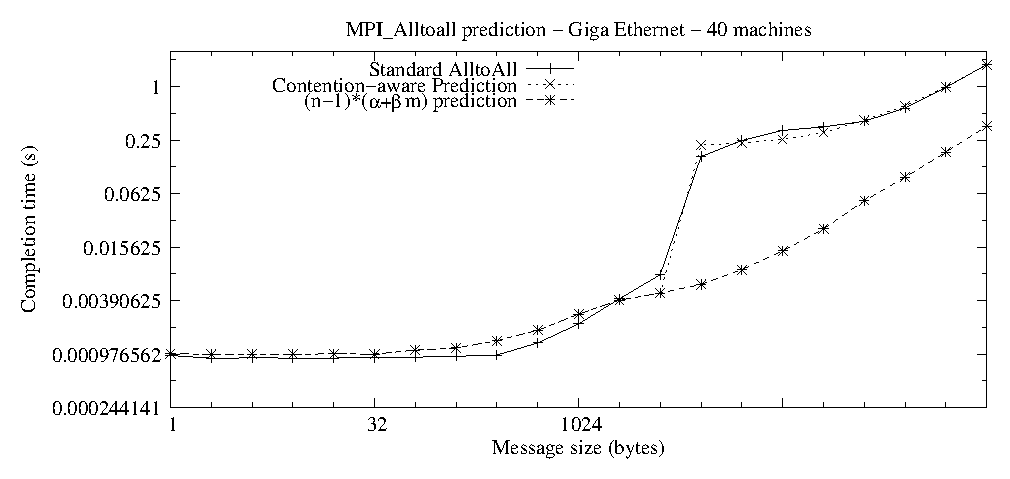
\includegraphics[width=0.7\columnwidth]{images/newcomp24_pred_log}
	\caption{\label{Figure: local}Performance mesurée et modélisée pour le MPI\_Alltoall dans un réseau Gigabit Ethernet}
\end{figure}


Vu la précision de ce modèle pour les \textit{clusters} homogènes, notre première réaction serait de l'appliquer aussi dans le cas des \textit{grids} de calcul en faisant la somme des performances des réseaux locaux et distants (Équation \ref{eq:7}). Malheureusement cette stratégie n'aboutit pas car les performances observées sont largement inférieures à celles prévues par ce modèle, comme indique la Figure \ref{Figure: standard}. 

\begin{equation}
T=max(T_{\mathcal C_1},T_{\mathcal C_2})+max(n_1, n_2) \times (\alpha_w+\beta_w \times m)
\label{eq:7}\end{equation}

En effet, la figure \ref{Figure: standard} représente des mesures effectuées entre deux \textit{clusters}, l'un situé à Nancy et l'autre à Rennes. Les deux \textit{clusters} étaient constitués de machines similaires (dual Opteron 246, 2 GHz) interconnectées localement par un réseau Gigabit Ethernet, alors que le lien \textit{inter-cluster} était un réseau privé de 10 Gbps. Les mesures ont été obtenues selon la méthode \emph{broadcast-barrier} \cite{Supinski99}.


\begin{figure}
	\centering
	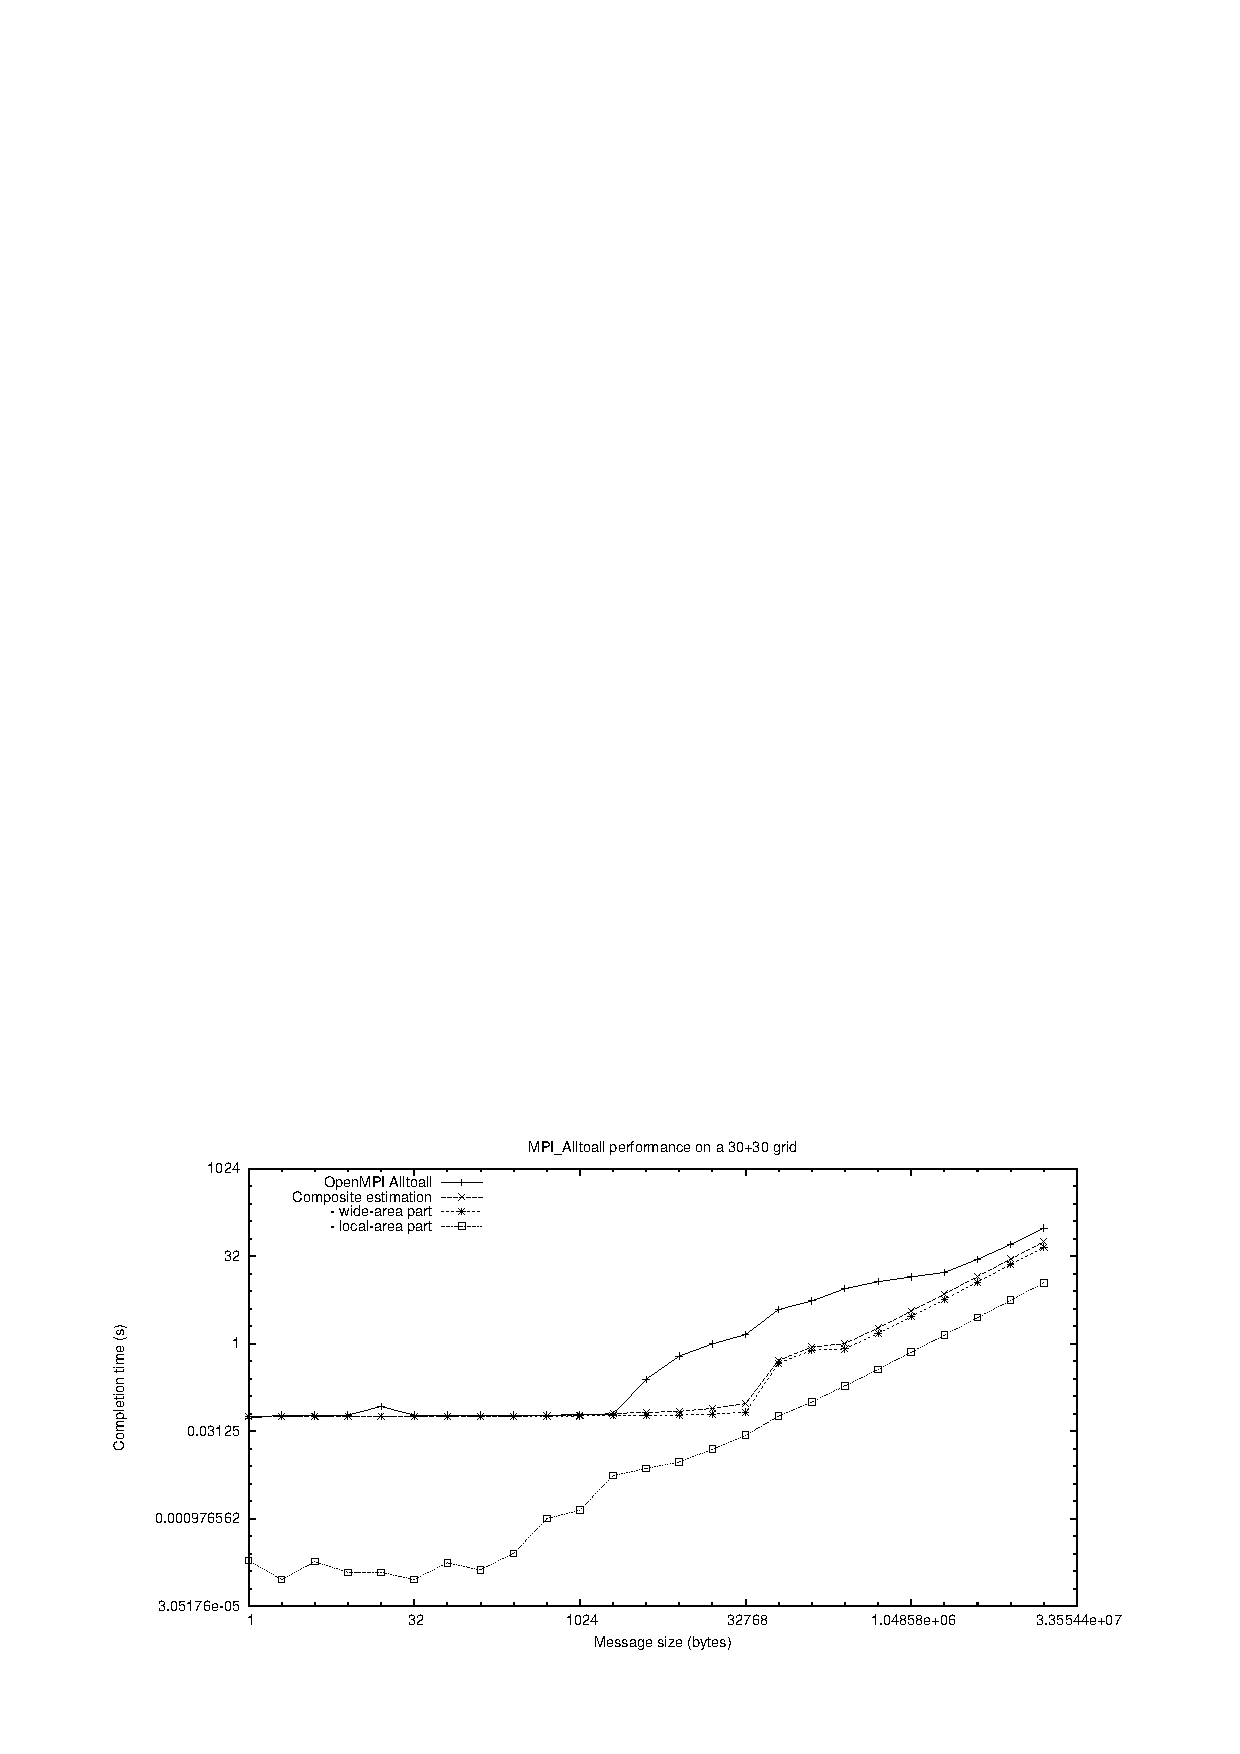
\includegraphics[width=0.7\columnwidth]{images/standard}
	%\vspace{-0.5cm}
	\caption{\label{Figure: standard}Performance mesurée et modélisée pour le MPI\_Alltoall dans un \textit{grid}} %\vspace{-0.5cm}
\end{figure}
 
Bien qu'on pourrait rajouter des paramètres supplémentaires pour s'approcher des performances observées, nous avons décidé d'attaquer le problème directement à sa source en optimisant la façon dont les communications sont effectuées sur un \textit{grid}. 


\subsection{All-to-All pour les \textit{Grids} : l'algorithme LG}

Lors de l'opération dans un \textit{grid}, l'un des facteurs les plus importants à prendre en compte est le temps nécessaire à ce que les messages soient livrés car ceux-ci sont affectés par la distance géographique mais aussi par l'hétérogénéité des protocoles, le routage des messages et les interférences des autres flux rencontrés sur le backbone. 

La plupart des algorithmes pour les communications collectives sur les \textit{grids} (PACX MPI~\cite{Gabriel98}, MagPIe~\cite{Kielmann01}) visent la minimisation des communications à grande distance en choisissant un coordinateur dans chaque \textit{cluster} qui sera responsable par les échanges \textit{intra-cluster}. Bien que ce mécanisme présente des avantages pour d'autres patrons de communication, il n'est pas adapté aux opérations de type  MPI\_Alltoall. En premier lieu, ce mécanisme  induit des étapes de communication supplémentaires du fait de forcer le passage par les coordinateurs des \textit{clusters}, qui de plus deviennent des goulots d'étranglement. En deuxième lieu, cette approche n'est pas optimale par rapport à l'utilisation des liens \textit{inter-cluster}, souvent capables de supporter des flux multiples \cite{Casanova05}. 

Afin de mieux traiter ce problème, nous essayons de minimiser les échanges distants d'une autre manière. En effet, la grande complexité des échanges du All-to-All réside dans les différentes performances des liens locaux et distants, or les implémentations traditionnelles de MPI\_Alltoall sont incapables de faire la différence. Si nous pouvons identifier la disposition des n{\oe}uds, on peut utiliser toutes les machines d'un \textit{cluster} pour collecter les données à un niveau local avant de les envoyer simultanément au réseau distant, en une unique étape de communication. 

Ainsi, le mécanisme que nous avons proposé en \cite{Steffenel07c} est une solution "\textit{grid aware}" qui s'exécute en deux étapes. Dans un premier moment, seulement les échanges locaux sont effectués. Cette phase inclut les échanges attendus entre les n{\oe}uds \textit{intra-cluster} mais aussi l'échange des données destinés aux autres \textit{clusters}, stockés dans des buffers supplémentaires pour la deuxième phase. L'avantage de cet échange est que son coût est très faible par rapport au coût d'une communication distante (voir Figure \ref{Figure: standard}). Finalement, lors de la deuxième phase, les buffers sont transmis directement aux n{\oe}uds destinataires, complétant ainsi l'échange total.  

Plus exactement, l'algorithme peut être décrit comme suit. Sans perte de généralité, considérons un \textit{cluster}  ${\mathcal C}_1$ qui contient moins de n{\oe}uds que le \textit{cluster} ${\mathcal C}_2$ ($n_1\leq n_2$). Les n{\oe}uds sont ainsi numérotés de 0 à $n_1+n_2-1$, avec les n{\oe}uds allant de 0 à $n_1-1$ appartenant à ${\mathcal C}_1$ et les n{\oe}uds allant de $n_1$ à $n_1+n_2-1$ appartenant au \textit{cluster} ${\mathcal C}_2$. Nous appelons ainsi ${\mathcal M}_{i,j}$ le message (donnée) qui sera envoyé du n{\oe}ud $i$ au n{\oe}ud $j$. 

L'algorithme suit les deux étapes : 
\begin{description}
	\item[Première étape] Pendant cette phase, nous effectuons les échanges locaux : Le n{\oe}ud $i$  envoie ${\mathcal M}_{i,j}$ au n{\oe}ud $j$, seulement si $i$ et $j$ font partie du même \textit{cluster}. Ensuite, ils préparent les buffers pour les communications distantes de manière à ce que les données à destination d'un n{\oe}ud distant $j$ on ${\mathcal C}_2$ seront d'abord stockés sur le n{\oe}ud $j~ mod~ n_1$ de ${\mathcal C}_1$. De même, les données sur un n{\oe}ud $i$ de ${\mathcal C}_2$ à destination de $j$ sur ${\mathcal C}_1$ seront stockés sur le n{\oe}ud $ \lfloor i/n_1 \rfloor \times n_1 + j $.
	\item[Deuxième étape] Pendant cette deuxième étape, seulement $n_2$ communications \textit{inter-cluster} auront lieu. Cette phase est décomposée en $\lceil n_2/n_1\rceil$ vagues avec $n_1$ communications chacune. Ainsi, pendant la vague $s$, le n{\oe}ud  $i$ de ${\mathcal C}_1$ échangera son buffer local avec le n{\oe}ud $j=i+n_1\times s$ de ${\mathcal C}_2$ (si $j < n_1+n_2$). Plus exactement, $i$ envoie  ${\mathcal M}_{k,j}$ à $j$ où $k\in [0,n_1]$ et $j$ envoie ${\mathcal M}_{k,i}$ à $i$ où $k\in[n_1\times s,n_1\times s+n_1-1]$.
\end{description}

Comme cet algorithme minimise le nombre de communications \textit{inter-cluster} et les organise par vagues, nous n'avons besoin que de $2\times \max(n_1,n_2)$ messages dans les deux directions (par rapport à  $2\times n_1 \times n_2$ messages dans l'algorithme traditionnel). Si les deux \textit{clusters} ont le même nombre de n{\oe}uds, une seule vague d'échanges sera nécessaire. Notre algorithme est aussi optimisé sur la longue distance car il regroupe plusieurs messages ensemble, réduisant l'impact de la latence et des interférences sur le backbone. La Figure \ref{Figure: comp} présente une comparaison entre la performance de l'algorithme traditionnel implémenté par OpenMPI et celle de l'implémentation de l'algorithme ${\mathcal LG}$. Nous observons que l'algorithme ${\mathcal LG}$ obtient un gain de performance de presque 50\% par rapport à la stratégie traditionnelle.

\begin{figure}
	\centering
	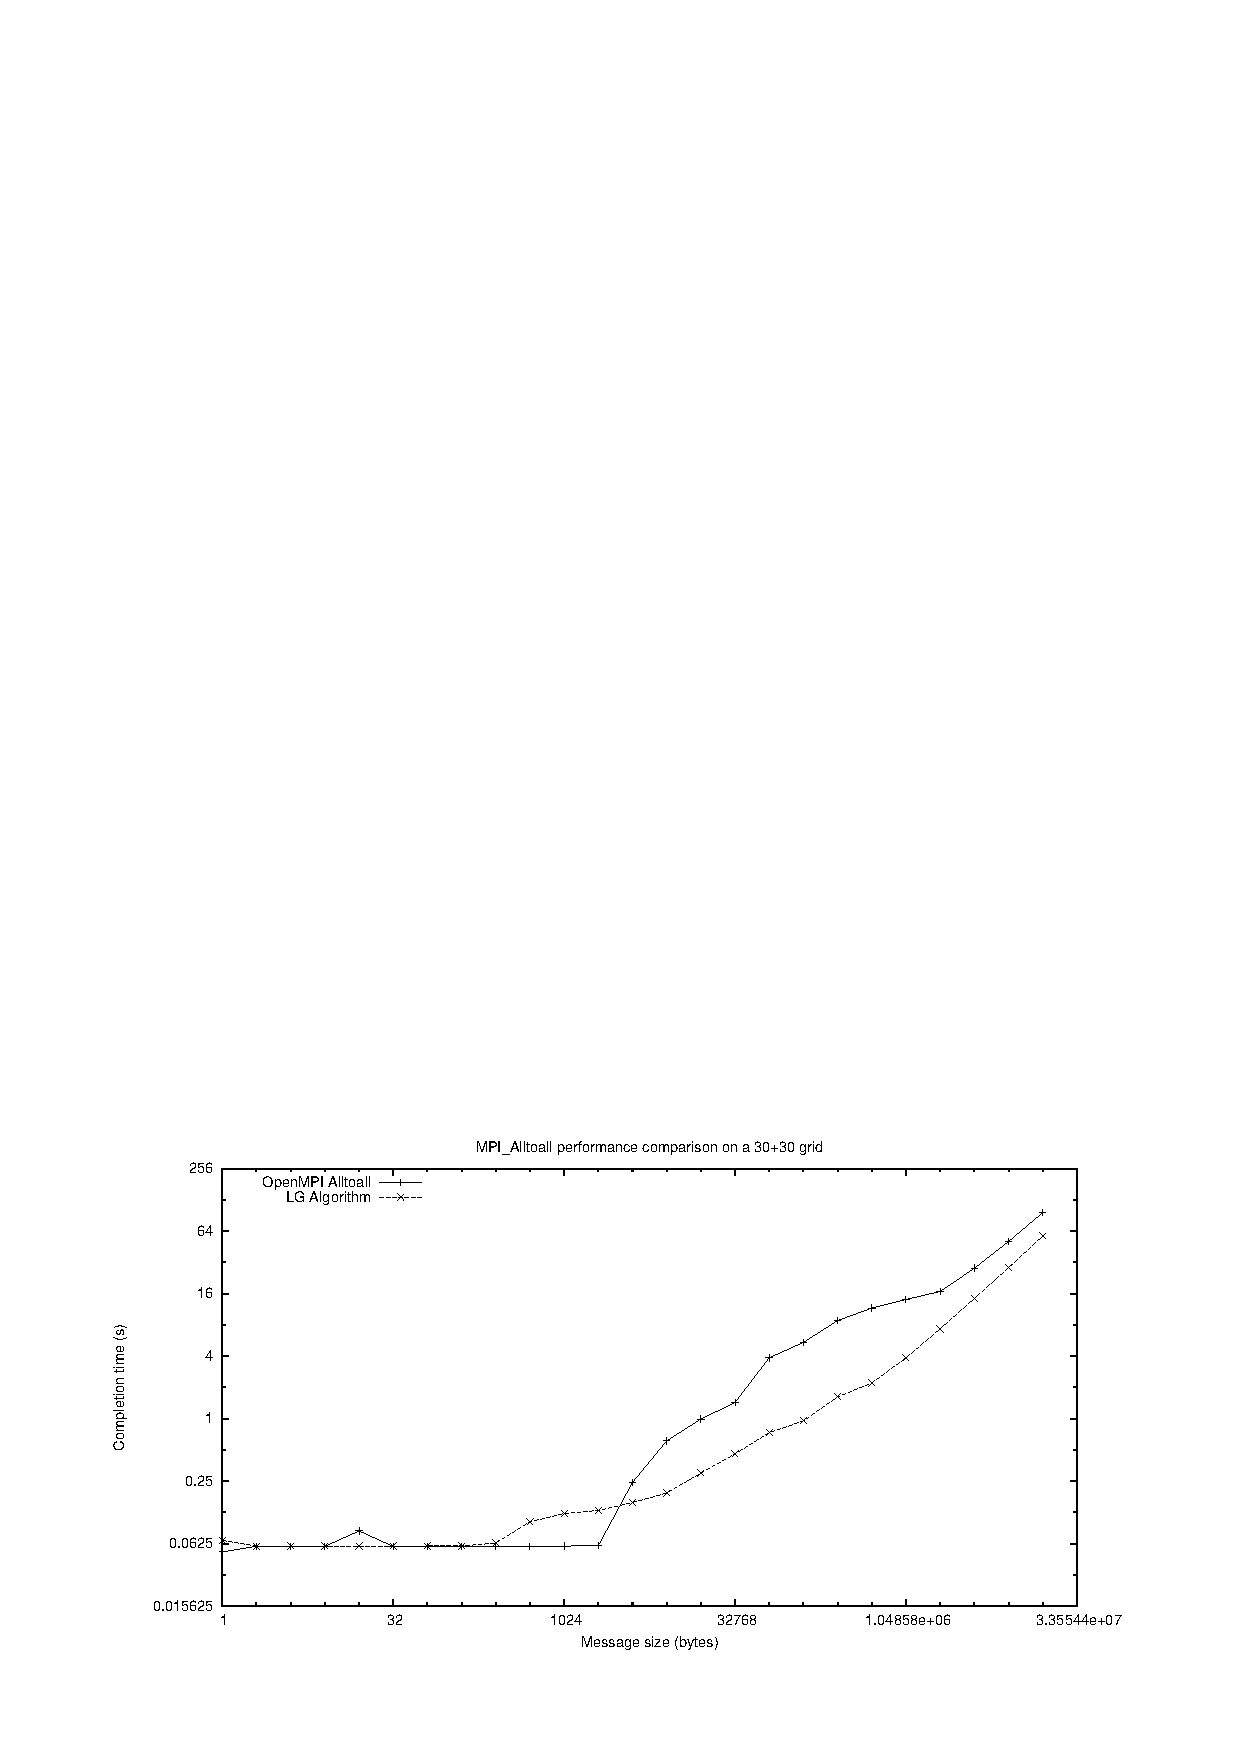
\includegraphics[width=0.7\columnwidth]{images/comp}
	\caption{\label{Figure: comp}Comparaison de performance entre OpenMPI et l'algorithme ${\mathcal LG}$}
\end{figure}

L'ordonnancement des communications effectué par ${\mathcal LG}$ a aussi une conséquence sur la modélisation des performances. Tout d'abord, il minimise les communications de longue distance, réduisant les risques de congestion qui sont difficiles de modéliser. De plus, la transmission groupée des messages réduit l'impact de la latence et des fluctuations de performance du réseau. C'est ainsi que nous avons pu établir un modèle composé des performances locales (${\mathcal T_{C_{n}}}$, obtenues à partir de l'équation \ref{eq:6}) et des prédictions pour les communications de longue distance obtenues par les méthodes traditionnelles :

\begin{equation}
T=max(T_{\mathcal C_1},T_{\mathcal C_2})+\lceil n_2/n_1\rceil \times (\alpha_w+\beta_w \times m \times n_1)
\label{eq:8}\end{equation}

Afin d'obtenir les paramètres nécessaires aux prédictions, nous avons utilisé la procédure décrite par Kielman \textit{et al.} \cite{Kielmann00}. Les facteurs de contention $\gamma=2.6887$ et $\delta=0.005039$ pour $M>=1KB$ ont été obtenus par la méthode des moindres carrés comme décrit par \cite{Steffenel06b}.

\begin{figure}
	\centering
		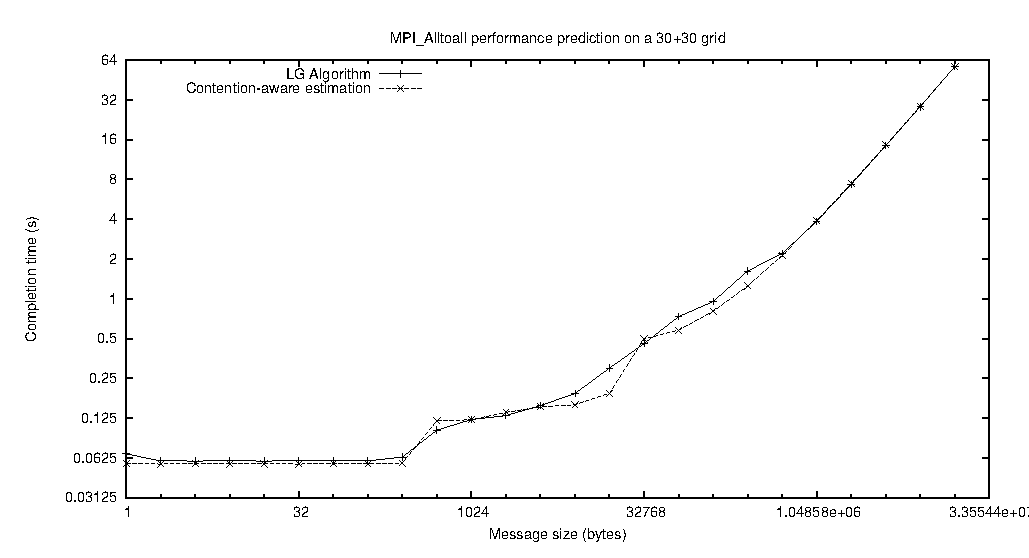
\includegraphics[width=0.7\columnwidth]{images/simul}
	\caption{\label{Figure: simul}Performance de ${\mathcal LG}$ et sa prédiction}
\end{figure}

La Figure \ref{Figure: simul} compare ainsi les prédictions obtenues avec l'Équation \ref{eq:8} et les performances mesurées pour l'algorithme ${\mathcal LG}$. Nous observons une bonne adéquation des prédictions, ce qui était impossible avec l'implémentation traditionnelle de MPI\_Alltoall. 

\section{Bilan et Perspectives}

Les travaux présentés dans ce chapitre prouvent l'intérêt de la modélisation des communications dans les réseaux hétérogènes, autant pour la prédiction des temps de communication que pour l'optimisation des algorithmes existants. Ceci est démontré notamment dans le cas de l'algorithme $LG$, qui a vu le jour uniquement parce que l'observation et la modélisation des performances indiquait des situations non-optimales dans les échanges entre deux \textit{clusters}.

Au fil des années mes intérêts se sont diversifiés et la modélisation des performances telles que présentées dans ce chapitre ne sont plus si fréquentes. Dans la plupart des cas mes travaux visent la comparaison des performances entre différentes approches logiciel et environnements d'exécution, ou bien l'amélioration des performances des applications grâce à la parallélisation de certaines routines. Ceci est le cas de deux travaux effectués récemment:

\subsubsection*{Utilisation de GPUs pour Augmenter la Performance d'une Application de \textit{Data Mining}}

Dans ces travaux effectués en collaboration avec Andrea Charão et Tiago Engel (Universidade Federal de Santa Maria, Brésil), nous nous sommes intéressés à l'optimisation des performances d'une application de \textit{data mining} et \textit{machine learning }très connue, Weka\footnote{\url{https://www.cs.waikato.ac.nz/ml/weka/}}. 

Bien que les termes \textit{data mining} et \textit{machine learning} soient fréquemment associés au \textit{big data}, on retrouve encore un nombre assez important d'applications et outils qui ne sont pas parallélisés ni s'exécutent sur un \textit{cluster} ou une infrastructure hébergée sur \textit{cloud}. Le plus souvent ceci est dû au fait que les masses de données ne sont pas tellement importantes pour avoir recours à des infrastructures plus puissantes, ou tout simplement car des instances moins importantes des données sont utilisées pour explorer et étudier un problème avant son déploiement.

Weka est un environnement très connu des chercheurs en \textit{data mining}, souvent utilisé pour l'apprentissage des techniques de classification, régression, clusterisation, etc. Weka est aussi une bibliothèque qui peut être intégrée aux application.  

Dans le cadre de ce travail nous avons constaté que la plupart des opérations sur Weka ne sont pas parallélisés (ni sur les multiples c{oe}urs de la CPU, ni sur un accélérateur GPU). En choissant les bonnes routines, nous croyons pouvoir améliorer sensiblement la performance de cette plateforme.

Grâce à l'étude des profiles d'exécutions lors de l'exécution d'une application métier (étude d'images de mammographie afin d'identifier des possibles sites tumoraux), nous avons pu déterminer un petit nombre d'opérations qui consommaient la plupart du temps de calcul. Ainsi, nous avons étudié le remplacement de ces opérations par des versions multi-c{oe}ur et GPU, avec comme résultat une réduction de plus de 50\% du temps d'exécution de l'application \cite{Engel14a,Engel2015}.

En ce moment nous poursuivons ces collaborations avec l'étude des performances d'accès aux services cloud \cite{Charao17a}  ou en associant des étudiants, comme par exemple les deux articles publiés récemment au Brésil (\cite{Nesi17a, Muenchen17a}) et conduits dans le cadre du projet de collaboration international CAPES-Cofecub MESO.

\subsubsection*{Évaluation des Performances de la Virtualisation sur les Dispositifs SoC (\textit{System on a Chip})}

Ce travail est le résultat d'une collaboration plus récente avec David Beserra, doctorant à l'Université Paris 1 sous l'encadrement de Manuele Kirsch-Pinheiro et Carine Souveyet. L'objectif ici est d'étudier les dispositifs SoC comme par exemple les Raspberry Pi, Banana Pi, etc. par rapport à leur capacité d'exécuter des machines virtuelles de type conteneur (par exemple LXC ou Docker). En effet, une application fréquemment citée pour ces dispositifs est celui de n{oe}ud de proximité dans un réseau \textit{fog computing}, et une meilleure compréhension du support à la virtualisation dans ces dispositifs peut aider le déploiement et la migration d'applications et de micro-services.

Des campagnes de mesure et d'analyse des performances ont été conduits lors de la première année de thèse de M Beserra, et ont donné lieu à deux publications dans des conférences internationales \cite{Beserra17a, Beserra17b}. La suite des travaux vise l'étude des plates-formes de micro-services, on espère bientôt pouvoir effectuer des nouvelles campagnes d'expérimentation.